%\documentclass[a4,semhelv,landscape]{seminar}
\documentclass[landscape]{slides}
%\documentclass[pdf, default, slideBW, nocolorBG]{prosper}
\usepackage[left=0.2cm,top=0.2cm,right=0.2cm,nohead,nofoot]{geometry}
%\def\everyslide{\sffamily}
%\usepackage{fullpage}
\usepackage{graphicx}
\usepackage[usenames]{color}
%\usepackage{color}
\usepackage{verbatim}
\usepackage{nopageno}
\usepackage{setspace}
%\usepackage{times}
% define some nice colors
\definecolor{myred}{rgb}{0.6,0,0}
\definecolor{myblue}{rgb}{0,0.2,0.4}
\definecolor{mygreen}{rgb}{0,0.5,0.0}
\definecolor{mypurple}{cmyk}{0.5,1.0,0.0,0.0}
%\color{myblue}

\begin{document}
%%%%%%%%%%%%%%%%%%%%%%%%%%%%%%%%%%%%%%%%%%%%%%%%%%%%%%%%%%%%%%%%%%%%
%Slide 0 - title
\begin{slide}
\begin{center}
\large{\textbf{Multiple alignment using sequence family profiles}}

\normalsize

Eric Nawrocki

Sean Eddy's Lab

\medskip

\medskip

\small

\begin{tabular}{c}
Howard Hughes Medical Institute \\ 
Janelia Farm Research Campus \\
\end{tabular}

\vspace{0.1in}


\includegraphics[width=2.5in]{figs/janelia-logo}
\end{center}
\end{slide}
%%%%%%%%%%%%%%%%%%%%%%%%%%%%%%%%%%%%%%%%%%%%%%%%%%%%%%%%%%%%%%%%%%%%
\begin{slide}
\begin{center}
\emph{De novo} \textbf{multiple sequence alignment methods assume very little}
\end{center}

\center{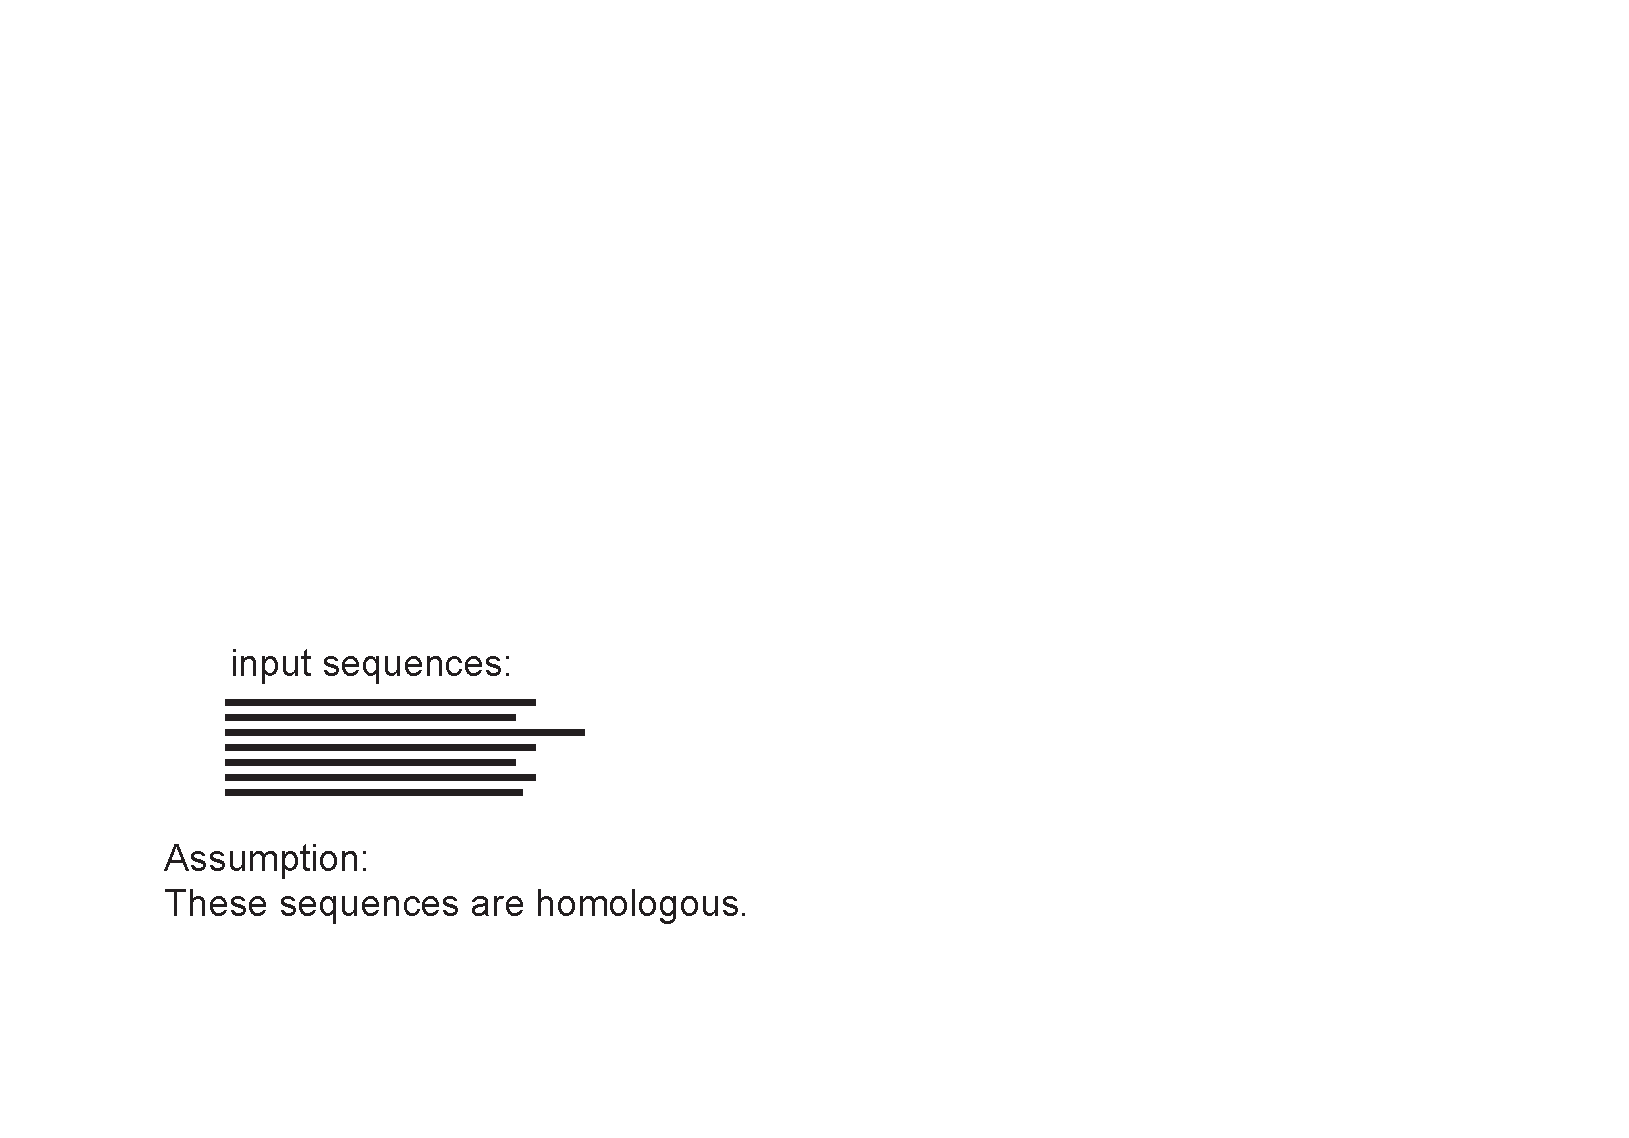
\includegraphics[width=10in]{figs/denovo-alignment-layer1}}

\vfill
\end{slide}
%%%%%%%%%%%%%%%%%%%%%%%%%%%%%%%%%%%%%%%%%%%%%%%%%%%%%%%%%%%%%%%%%%%%
\begin{slide}
\begin{center}
\emph{De novo} \textbf{multiple sequence alignment methods assume very little}
\end{center}

\center{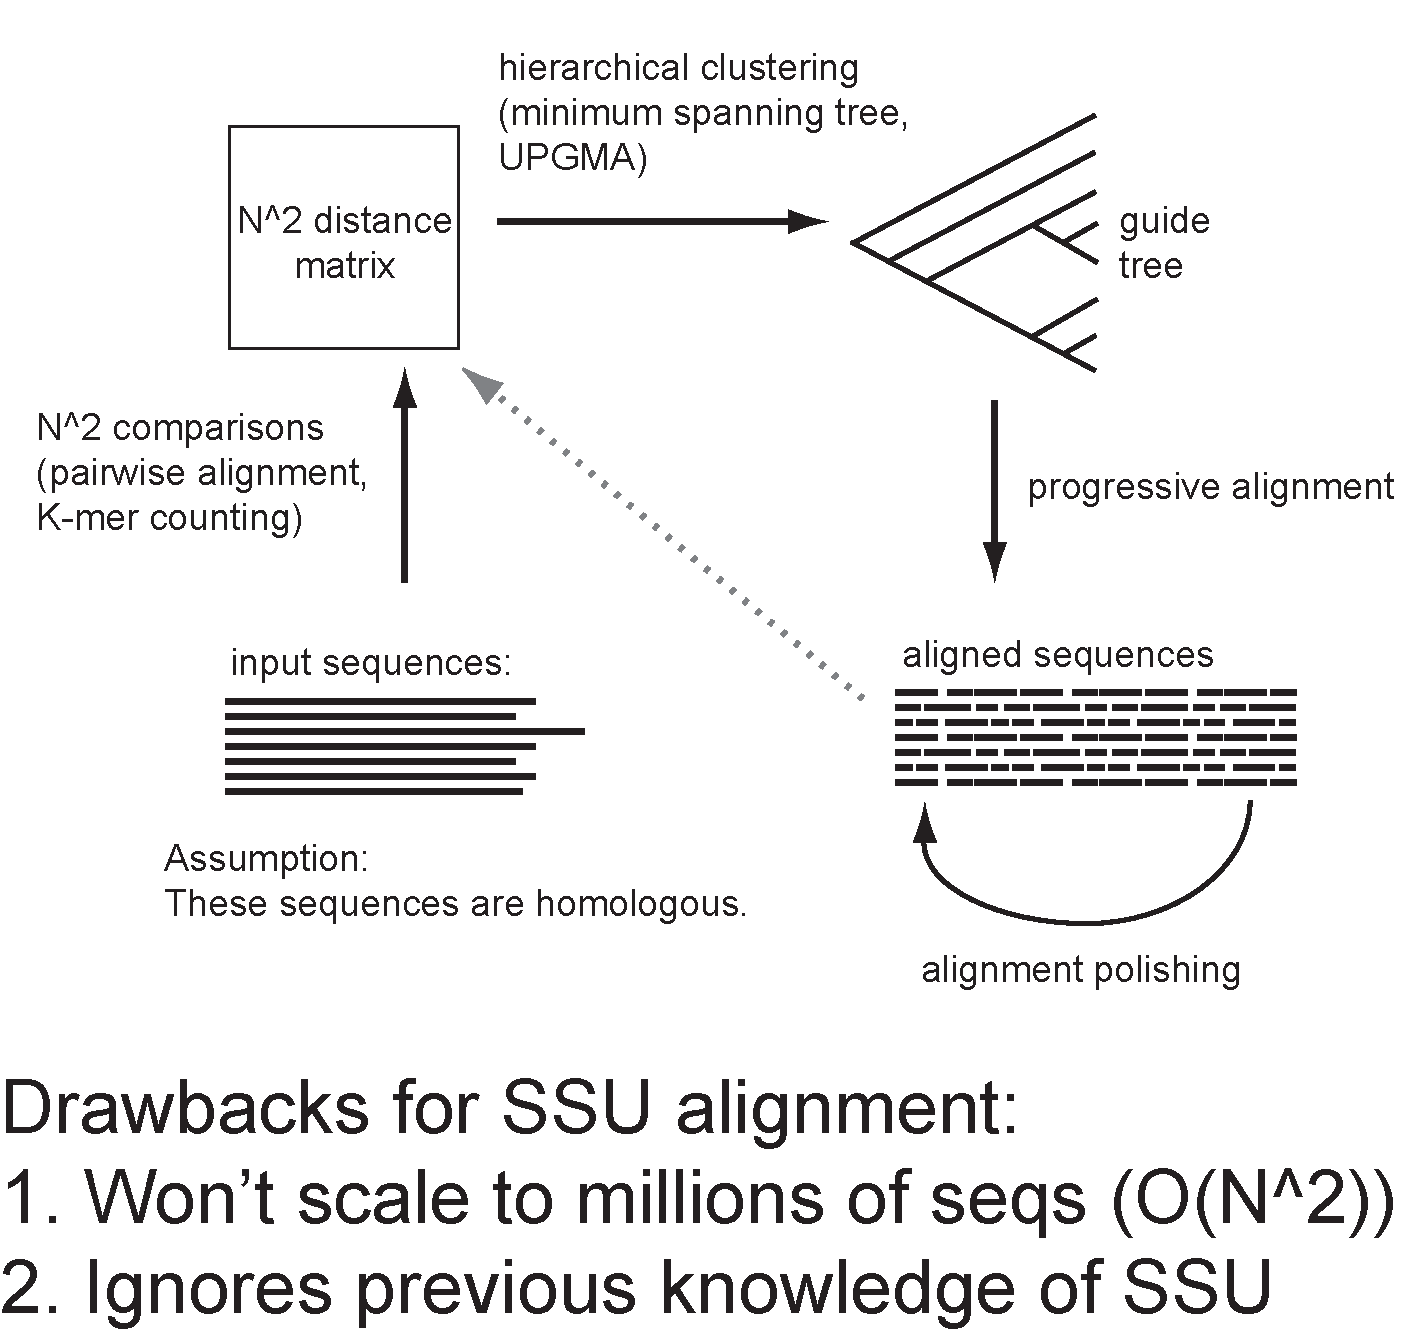
\includegraphics[width=10in]{figs/denovo-alignment}}

\vfill
\end{slide}
%%%%%%%%%%%%%%%%%%%%%%%%%%%%%%%%%%%%%%%%%%%%%%%%%%%%%%%%%%%%%%%%%%%%
\begin{slide}
\begin{center}
\textbf{A trusted (probably manually curated) reference alignment can help}
\end{center}

\small
\begin{itemize} 
\item Usually we're aligning sequences of a known family (e.g. 16S/18S SSU rRNA).
\item Assume we have a reference alignment that is \emph{correct} and \emph{representative}.
\item Advantages versus \emph{de novo}: 
\begin{itemize} 
  \item $O(NM)$ for $N$ new sequences and $M$ sequences in reference
  alignment
  \item potentially more accurate final alignment, due to trusted
  starting point
\end{itemize}
\end{itemize}

\vfill
\end{slide}
%%%%%%%%%%%%%%%%%%%%%%%%%%%%%%%%%%%%%%%%%%%%%%%%%%%%%%%%%%%%%%%%%%%%
\begin{slide}
\begin{center}
\textbf{Nearest-neighbor-based versus Profile-based reference alignment}
\end{center}

\center{\includegraphics[width=10in]{figs/reference-alignment-nn-v-profile-layer1}}

\vfill
\end{slide}
%%%%%%%%%%%%%%%%%%%%%%%%%%%%%%%%%%%%%%%%%%%%%%%%%%%%%%%%%%%%%%%%%%%%
\begin{slide}
\begin{center}
\textbf{Nearest-neighbor-based versus Profile-based reference alignment}
\end{center}

\center{\includegraphics[width=10in]{figs/reference-alignment-nn-v-profile-layer2}}

\vfill
\end{slide}
%%%%%%%%%%%%%%%%%%%%%%%%%%%%%%%%%%%%%%%%%%%%%%%%%%%%%%%%%%%%%%%%%%%%
\begin{slide}
\begin{center}
\textbf{Profiles have position-specific scores \\ (substitutions, gap
    open, gap extend}
\end{center}

\center{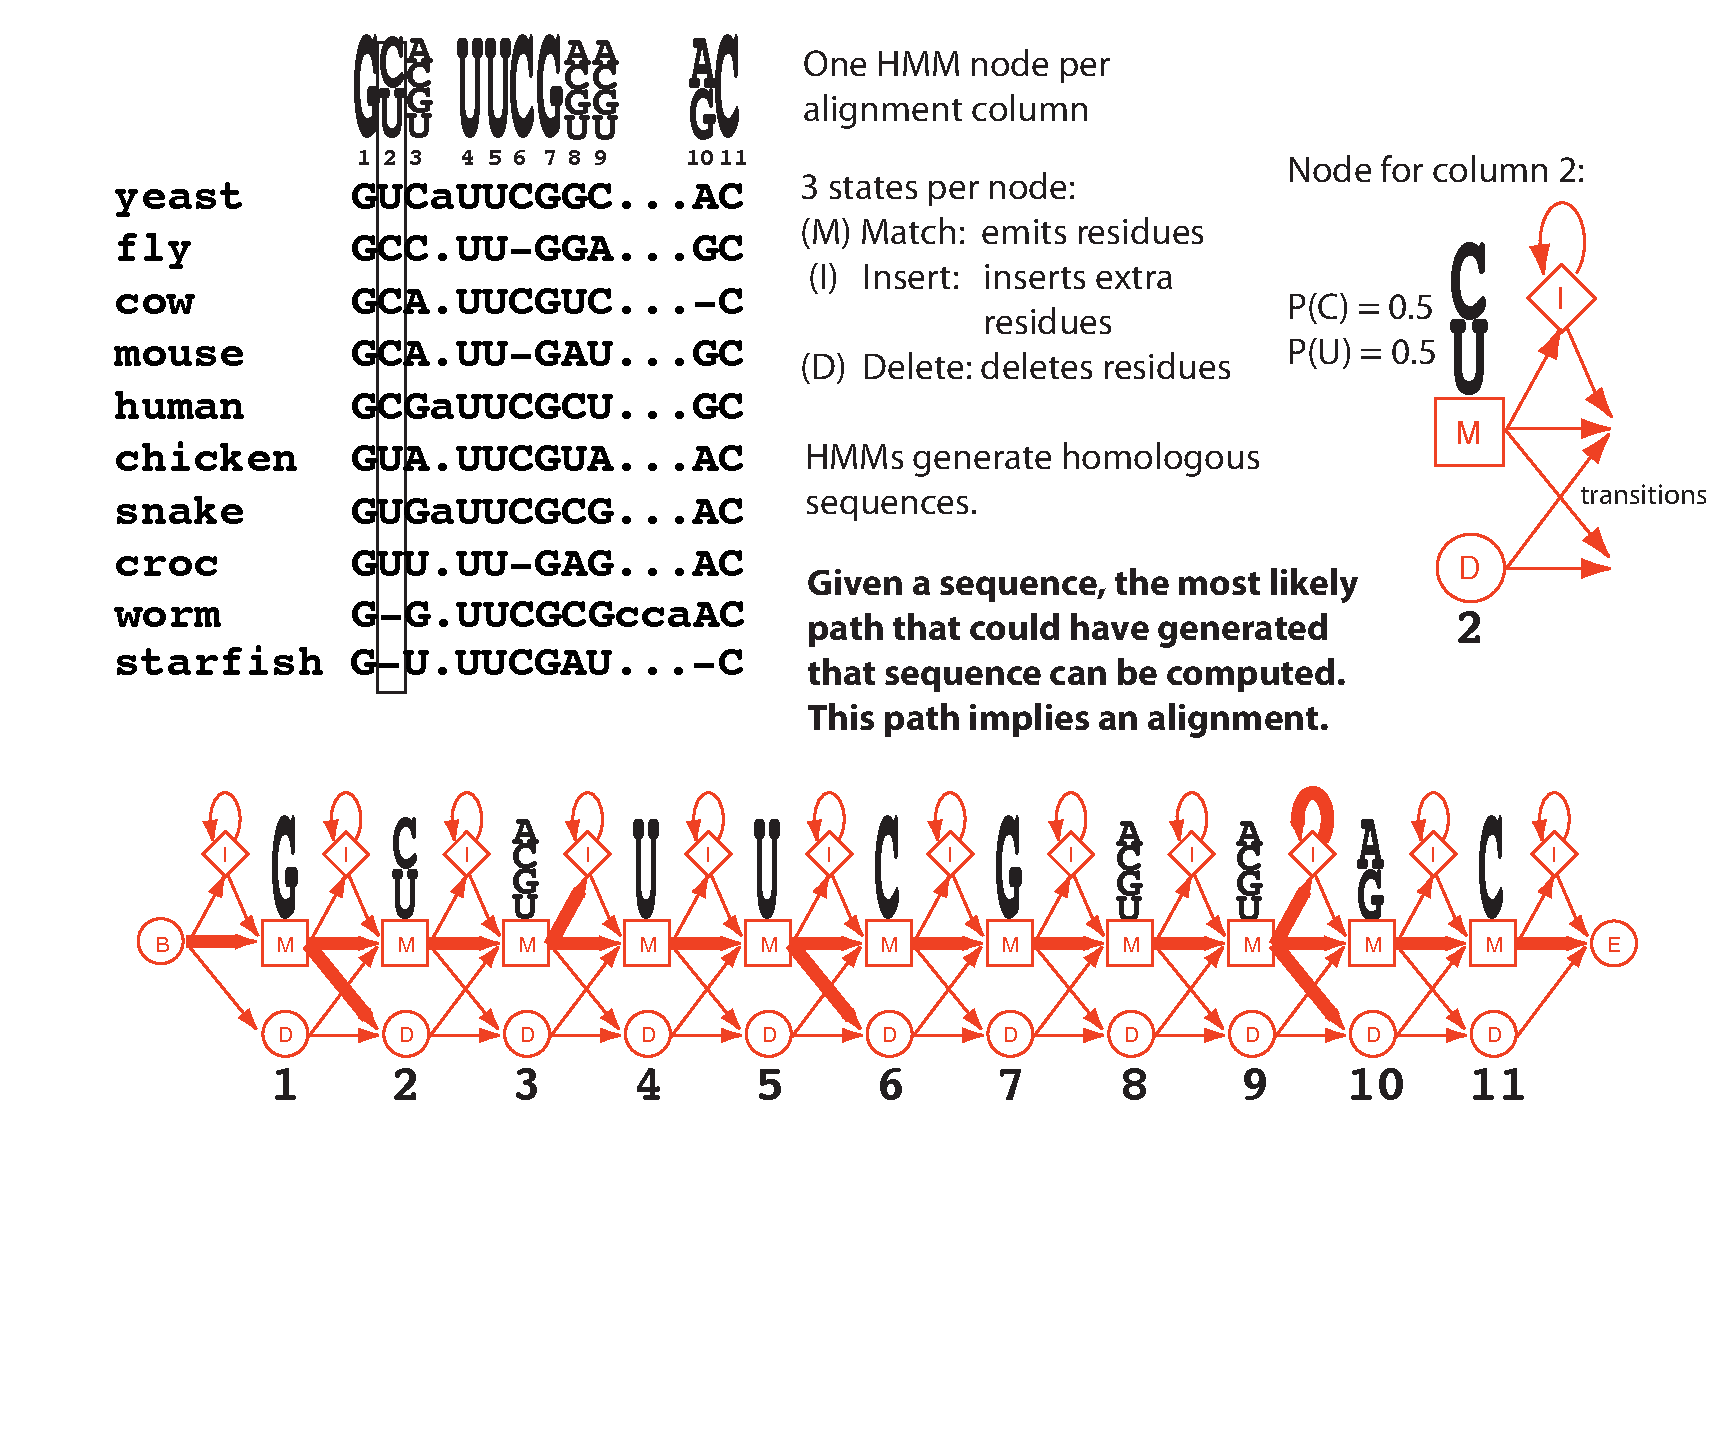
\includegraphics[height=6in]{figs/alignment-hmm-layer1}}

\vfill
\end{slide}
%%%%%%%%%%%%%%%%%%%%%%%%%%%%%%%%%%%%%%%%%%%%%%%%%%%%%%%%%%%%%%%%%%%%
\begin{slide}
\begin{center}
\textbf{Profiles HMMs are probabilistic profiles built from alignments}
\end{center}

\center{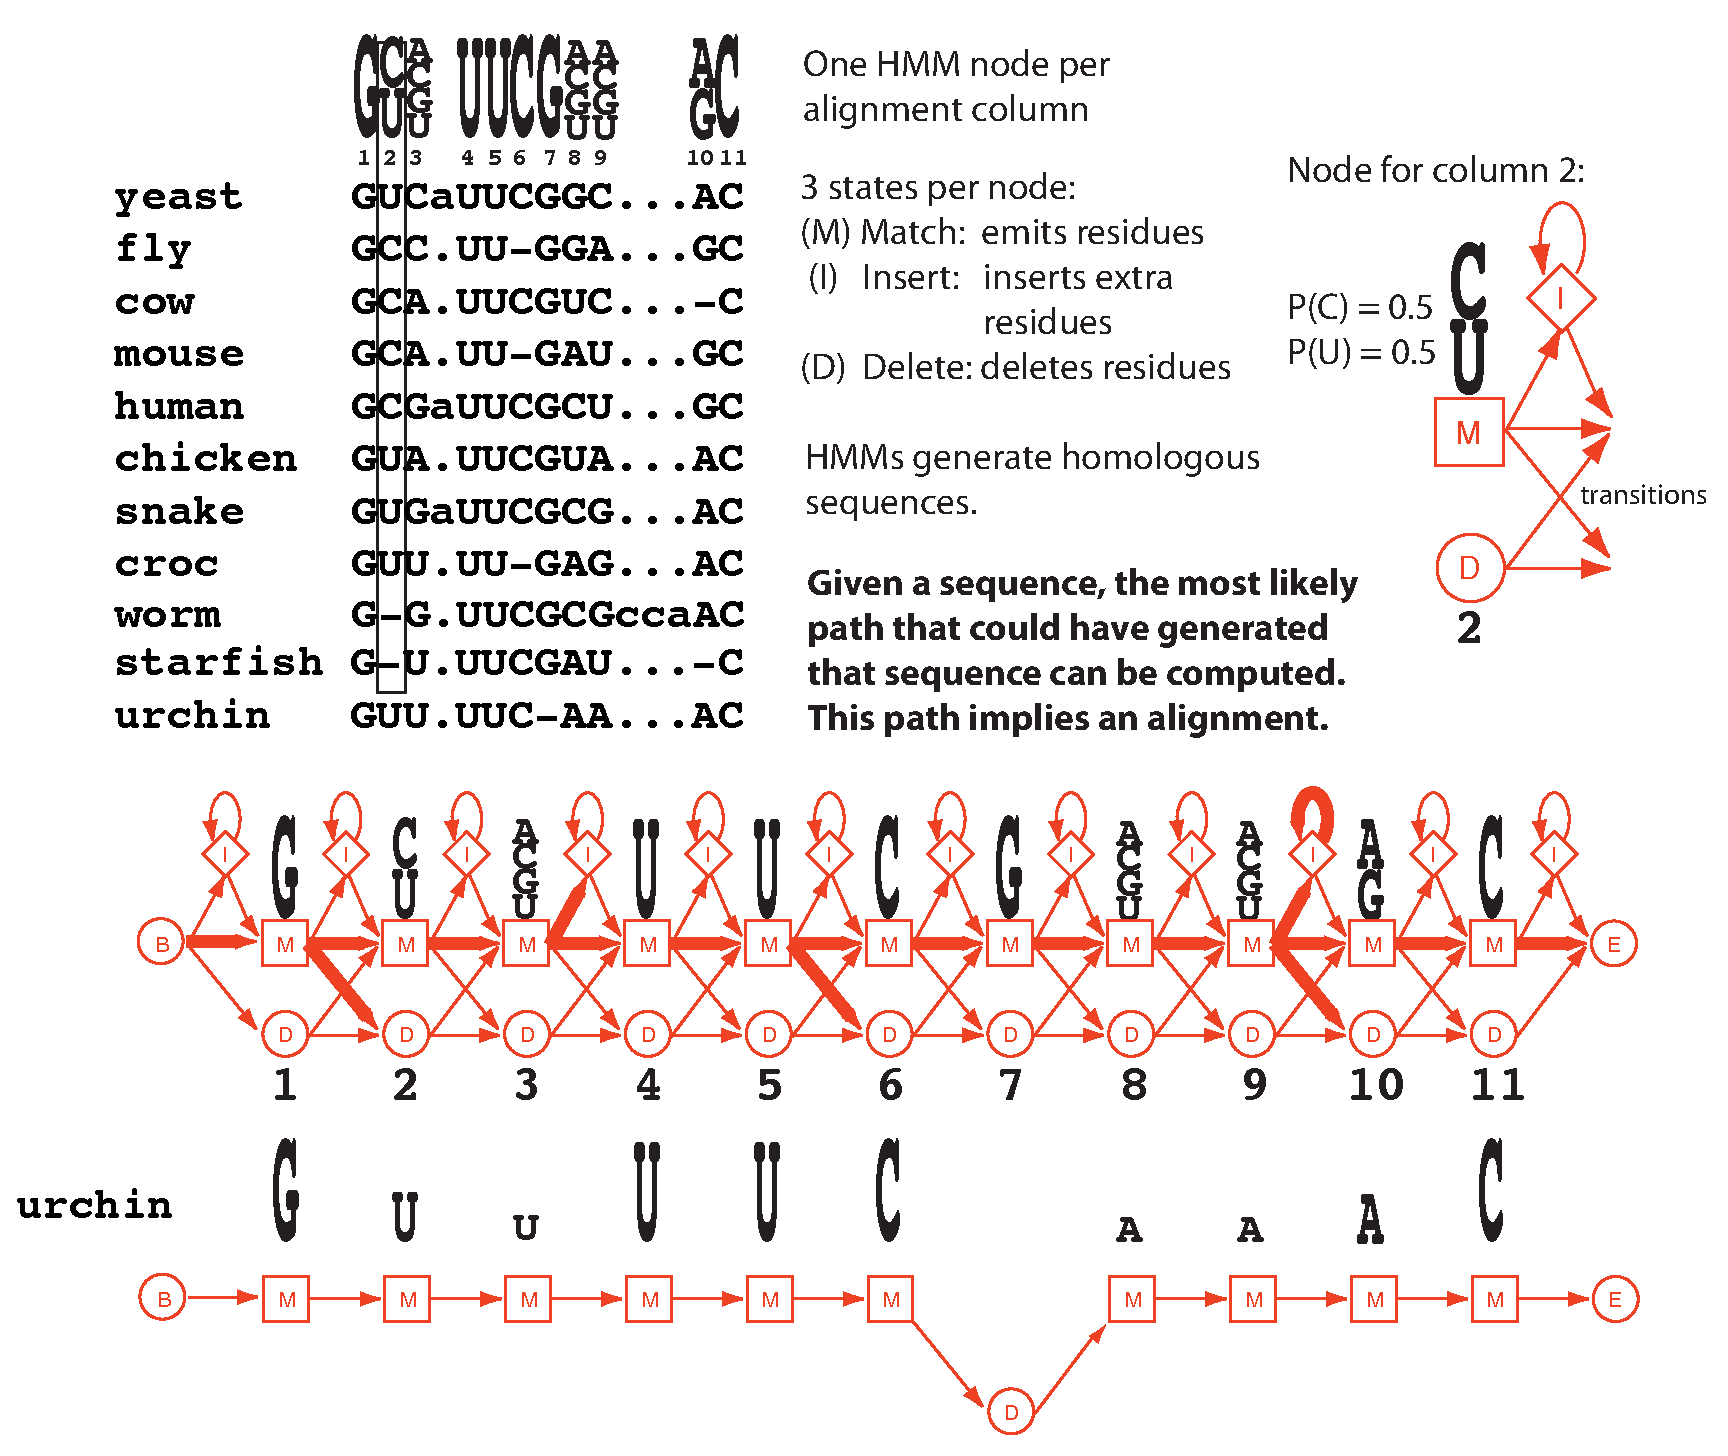
\includegraphics[height=6in]{figs/alignment-hmm-layer2}}

\vfill
\end{slide}
%%%%%%%%%%%%%%%%%%%%%%%%%%%%%%%%%%%%%%%%%%%%%%%%%%%%%%%%%%%%%%%%%%%%
\begin{slide}
\begin{center}
\textbf{Sequences are aligned to profiles HMMs using dynamic
  programming algorithms very similar to Smith-Waterman}
\end{center}

\center{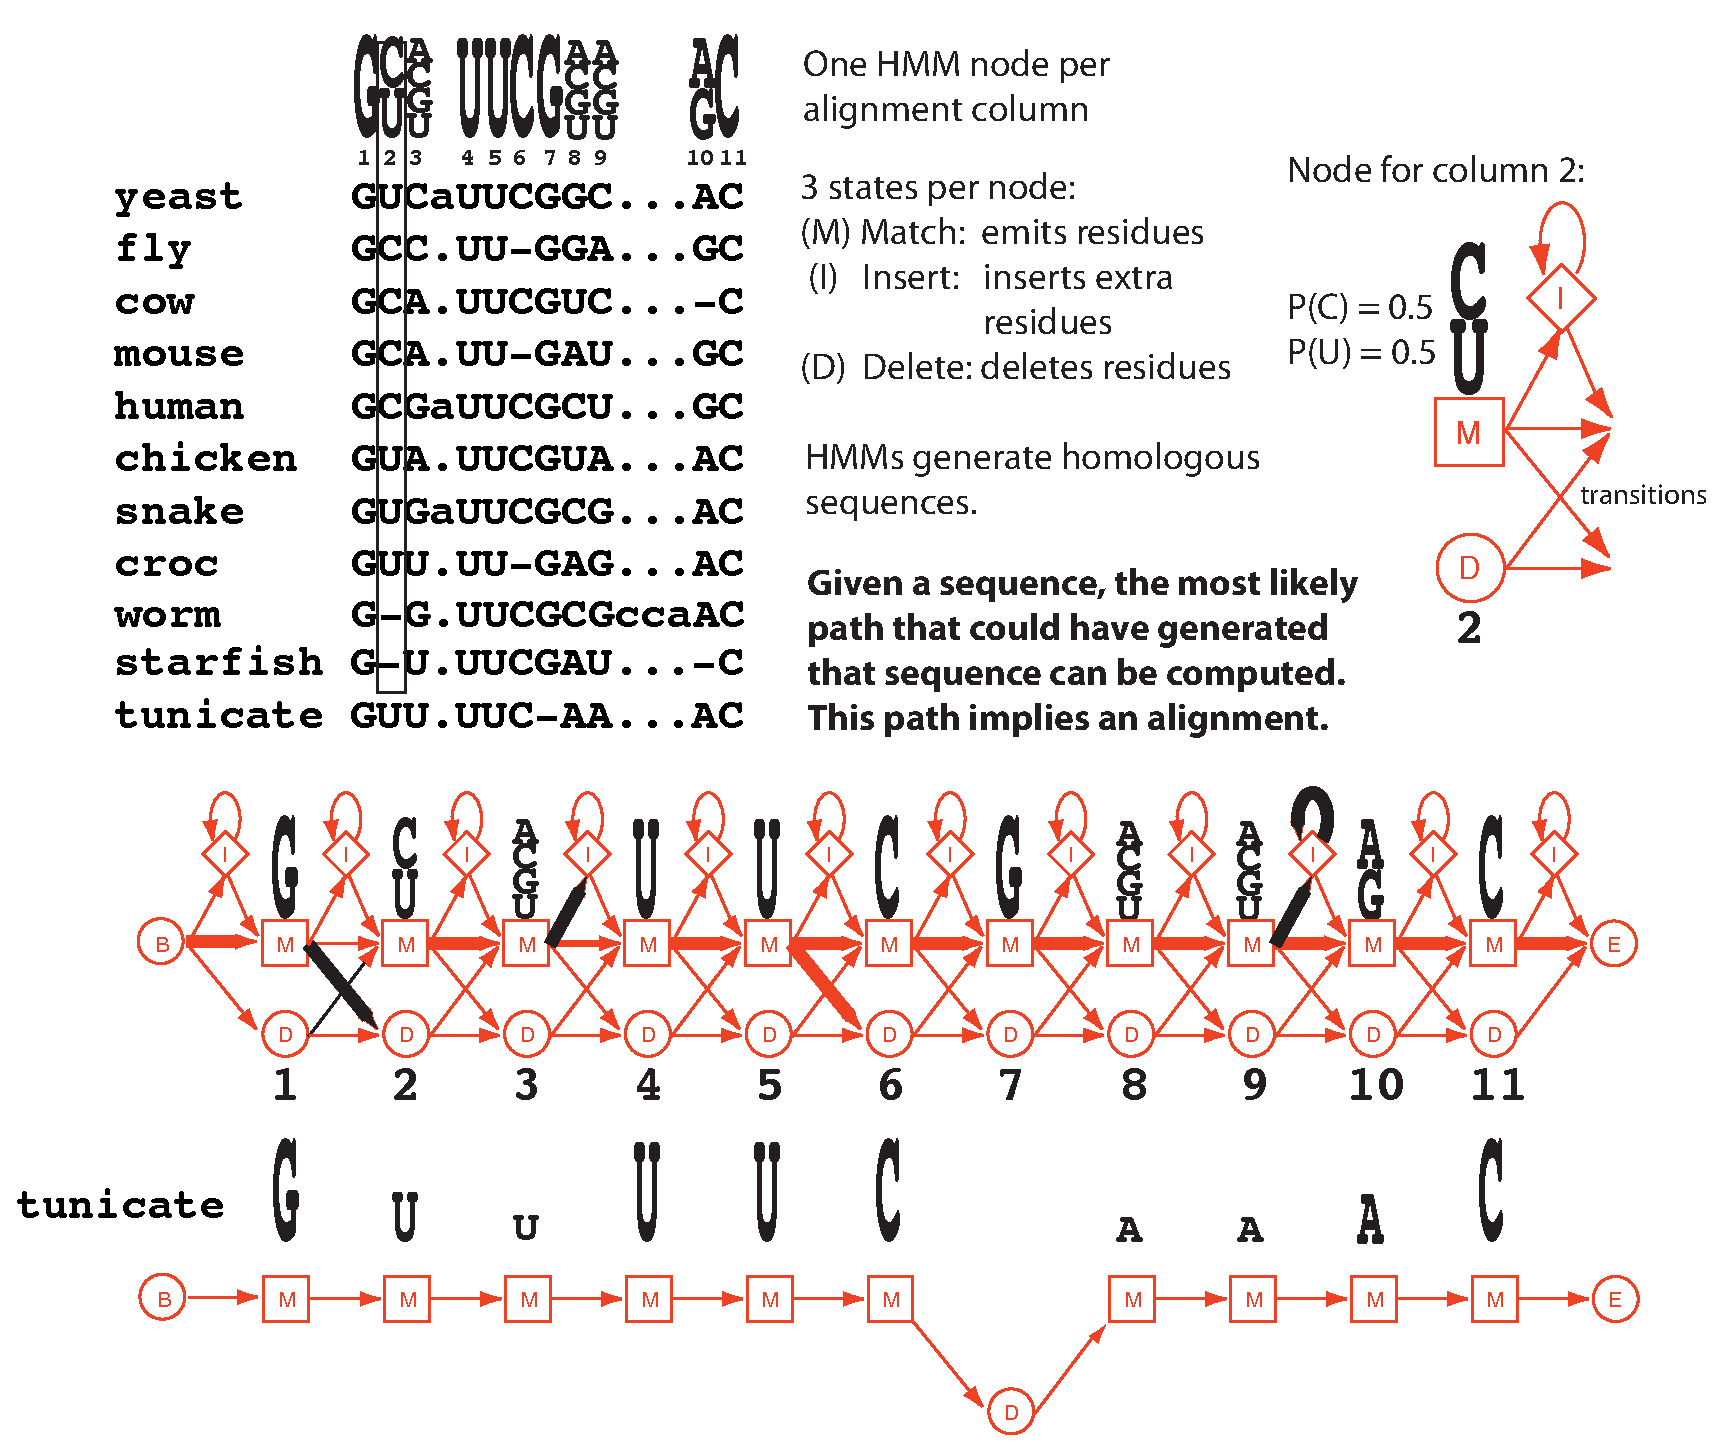
\includegraphics[height=6in]{figs/alignment-hmm-layer3}}

\vfill
\end{slide}
%%%%%%%%%%%%%%%%%%%%%%%%%%%%%%%%%%%%%%%%%%%%%%%%%%%%%%%%%%%%%%%%%%%%
\begin{slide}
\begin{center}
\textbf{Profiles can be more accurate than pairwise alignment}
\end{center}

\center{\includegraphics[width=9in]{figs/nn-pairwise-example}}

\vfill
\end{slide}
%%%%%%%%%%%%%%%%%%%%%%%%%%%%%%%%%%%%%%%%%%%%%%%%%%%%%%%%%%%%%%%%%%%%
\begin{slide}
\begin{center}
\textbf{Conservation levels and insertion frequency vary in SSU rRNA}
\end{center}

\begin{center}
\includegraphics[height=6.5in]{figs/bacteria-0p1-info}
\includegraphics[height=6.5in]{figs/bacteria-0p1-ifreq}
\end{center}

\vfill
\end{slide}
%%%%%%%%%%%%%%%%%%%%%%%%%%%%%%%%%%%%%%%%%%%%%%%%%%%%%%%%%%%%%%%
\begin{slide}
\begin{center}
%\textbf{profile HMMs and covariance models}
\textbf{Covariance models (CMs) are built \\ from structure-annotated alignments}
\end{center}
\medskip

\center{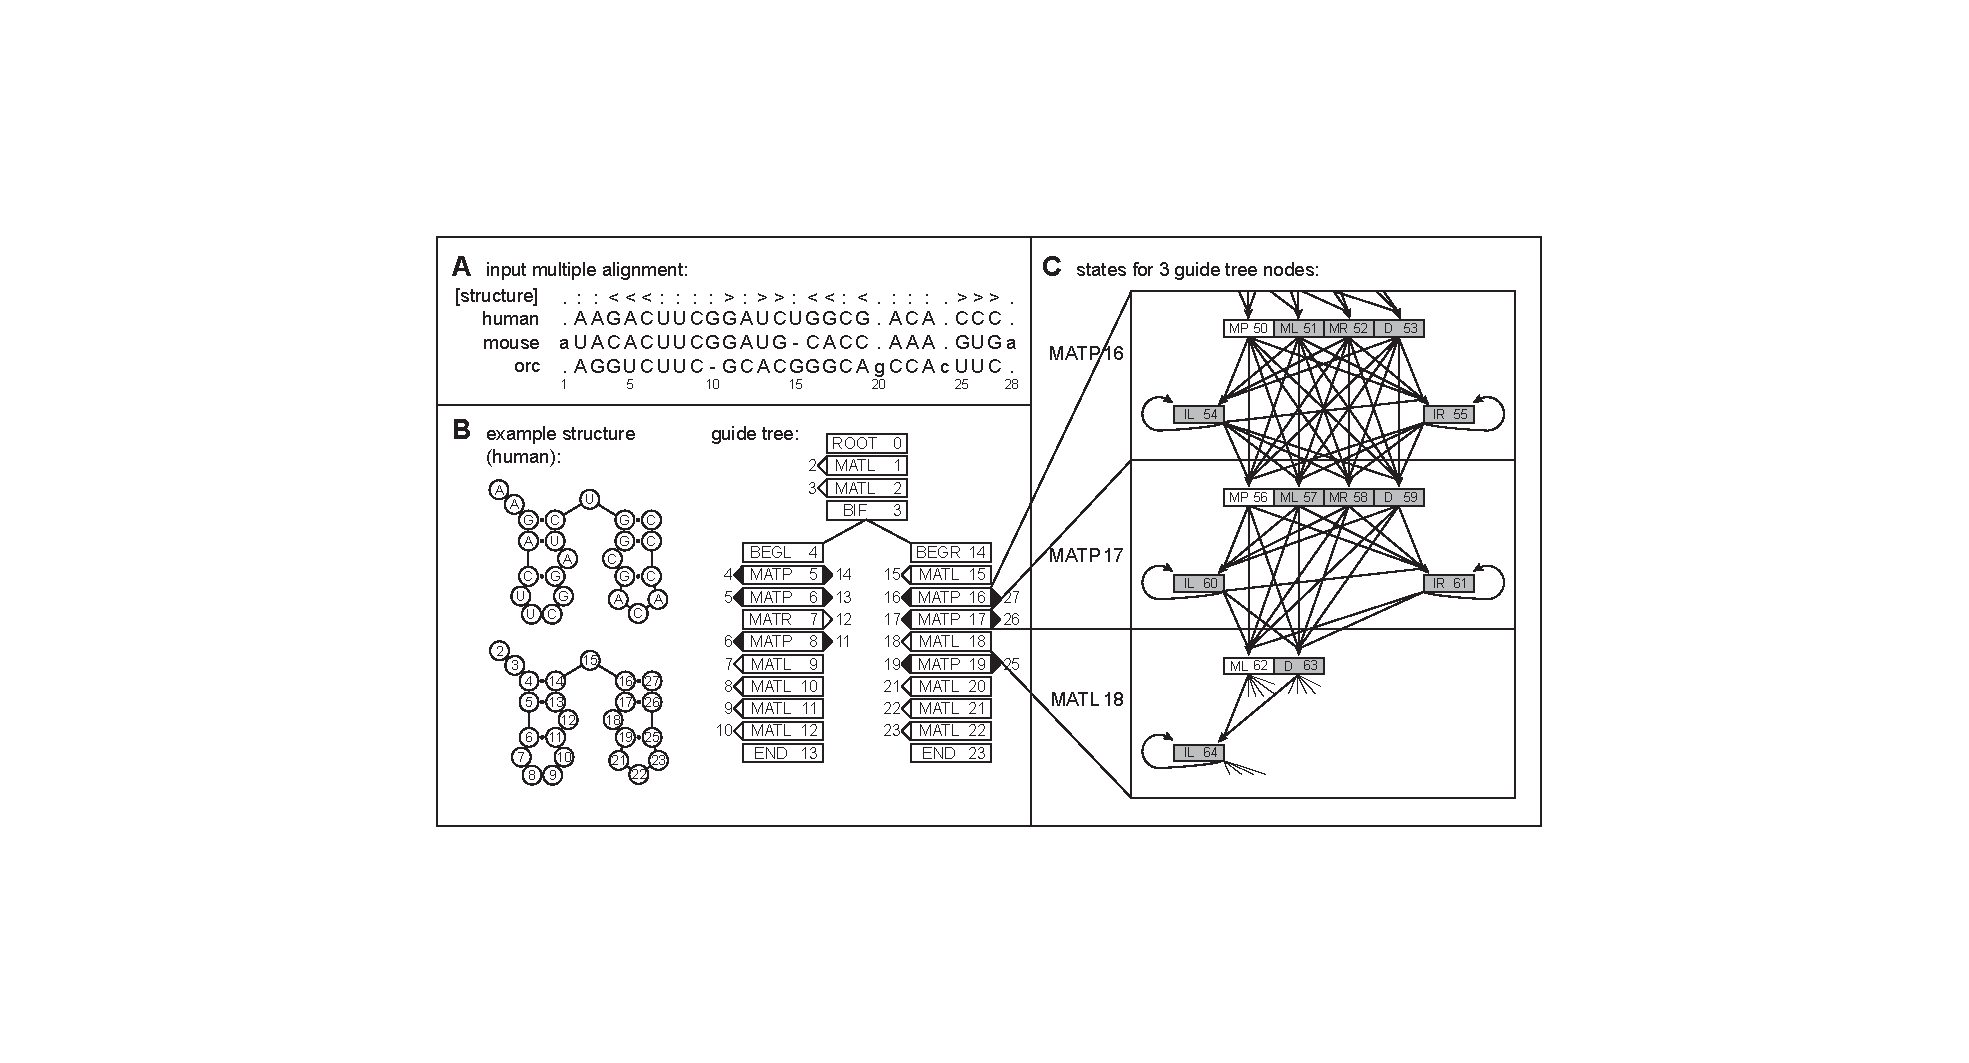
\includegraphics[width=8in]{figs/cmintro_bandcyk}}

\center{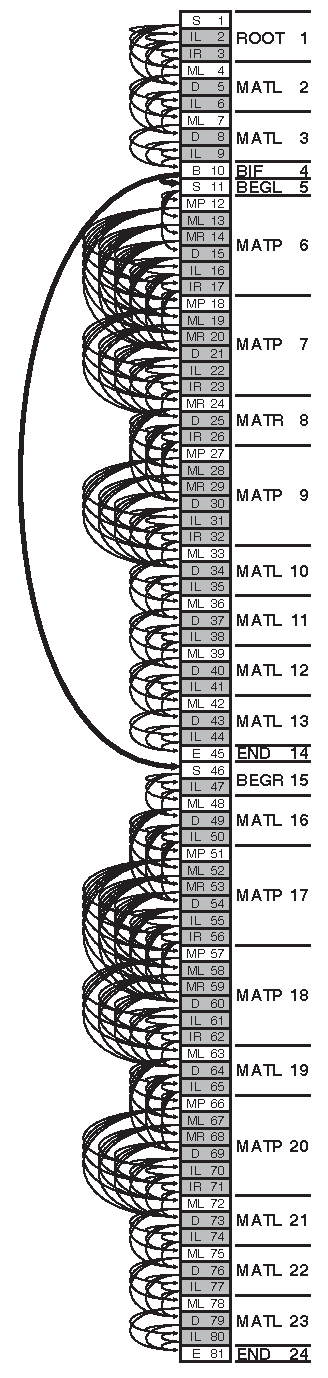
\includegraphics[width=2in,angle=270]{figs/cm-graph-small}}

%\item Extensions of profile HMMs that 

%\item Generative models that generate ``homologous'' structural RNA sequences

\vfill

\end{slide}
%%%%%%%%%%%%%%%%%%%%%%%%%%%%%%%%%%%%%%%%%%%%%%%%%%%%%%%%%%%%%%%%%%%%
\begin{slide}
\begin{center}
\textbf{Benchmark of SSU alignment}
\end{center}
\medskip

\small
\begin{itemize}
\item
How accurate are profile-based alignments?
\item
'Gold standard' testing dataset
\begin{itemize}
\item
structural alignment of 152 bacterial SSU sequences
from Robin Gutell's database
\item
this is the CRW bacterial seed alignment filtered to 92\% identity
\item
determined by 'manual' comparative analysis
\end{itemize}
\end{itemize}

\center{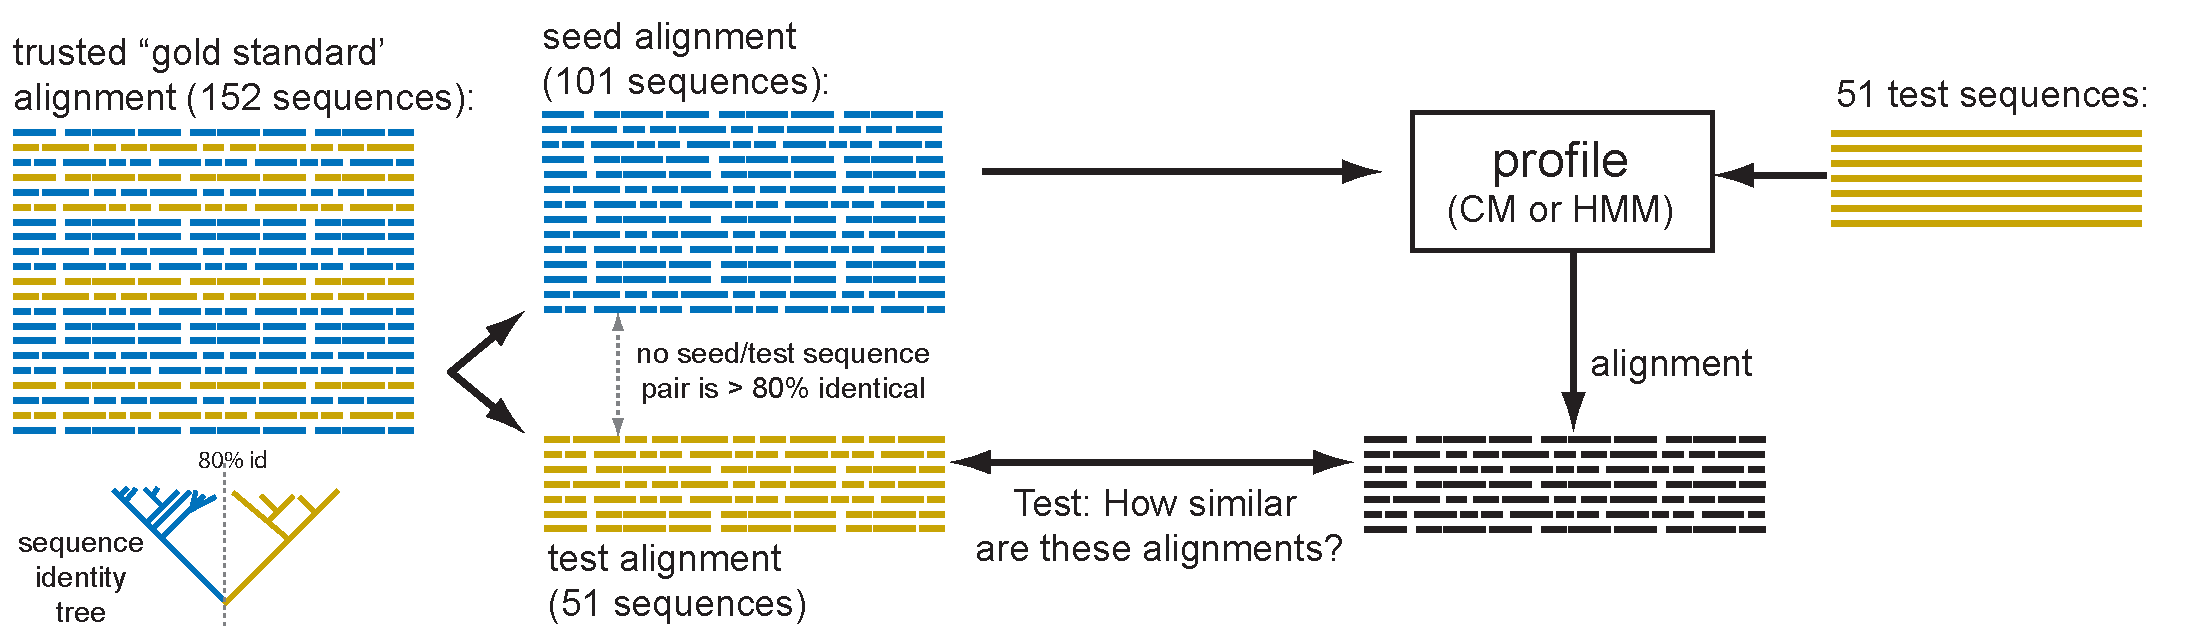
\includegraphics[width=10.5in]{figs/diana_benchmark_l2}}

\vfill
\end{slide}
%%%%%%%%%%%%%%%%%%%%%%%%%%%%%%%%%%%%%%%%%%%%%
\begin{slide}
\begin{center}
\textbf{Profiles produce accurate SSU alignments}
\end{center}
\medskip
\medskip
\begin{center}

\begin{tabular}{rcr} 
& \multicolumn{1}{c}{alignment} & \multicolumn{1}{c}{time} \\
& \multicolumn{1}{c}{accuracy} & \multicolumn{1}{c}{(sec/seq)} \\ \hline
& \multicolumn{1}{c}{} & \multicolumn{1}{c}{} \\
clustalw & 92.2\% & 30.0 \\ 
& \multicolumn{1}{c}{} & \multicolumn{1}{c}{} \\
HMMs & 96.6\% & 0.08 \\ 
& \multicolumn{1}{c}{} & \multicolumn{1}{c}{} \\
non-banded CMs & 98.1\% & 1321.5 \\ 
& \multicolumn{1}{c}{} & \multicolumn{1}{c}{} \\
HMM banded CMs & 98.1\% & 0.7 \\ %1.1
& \multicolumn{1}{c}{} & \multicolumn{1}{c}{} \\
\end{tabular}
\end{center}

\vfill
\end{slide}
%%%%%%%%%%%%%%%%%%%%%%%%%%%%%%%%%%%%%%%%%%%%%%%%%%%%%%%%%%%%%%%%%%%%%%%%%
\begin{slide}
\begin{center}
\textbf{Benefits of using probabilistic models: two examples}
\end{center}

\begin{enumerate} 
\item HMM banding: calculation of dynamic programming matrix bands for
  faster CM alignment.
\item Posterior probabilities of each aligned residue: useful for
  identifying and masking columns that are not reliably
  aligned. 
\end{enumerate}

\vfill
\end{slide}
%%%%%%%%%%%%%%%%%%%%%%%%%%%%%%%%%%%%%%%%%%%%%%%%%%%%%%%%%%%%%%%%%%%%%%%%%%
\begin{slide}
\begin{center}

%\large
\textbf{Using SSU as a phylogenetic marker}
\end{center}

\center{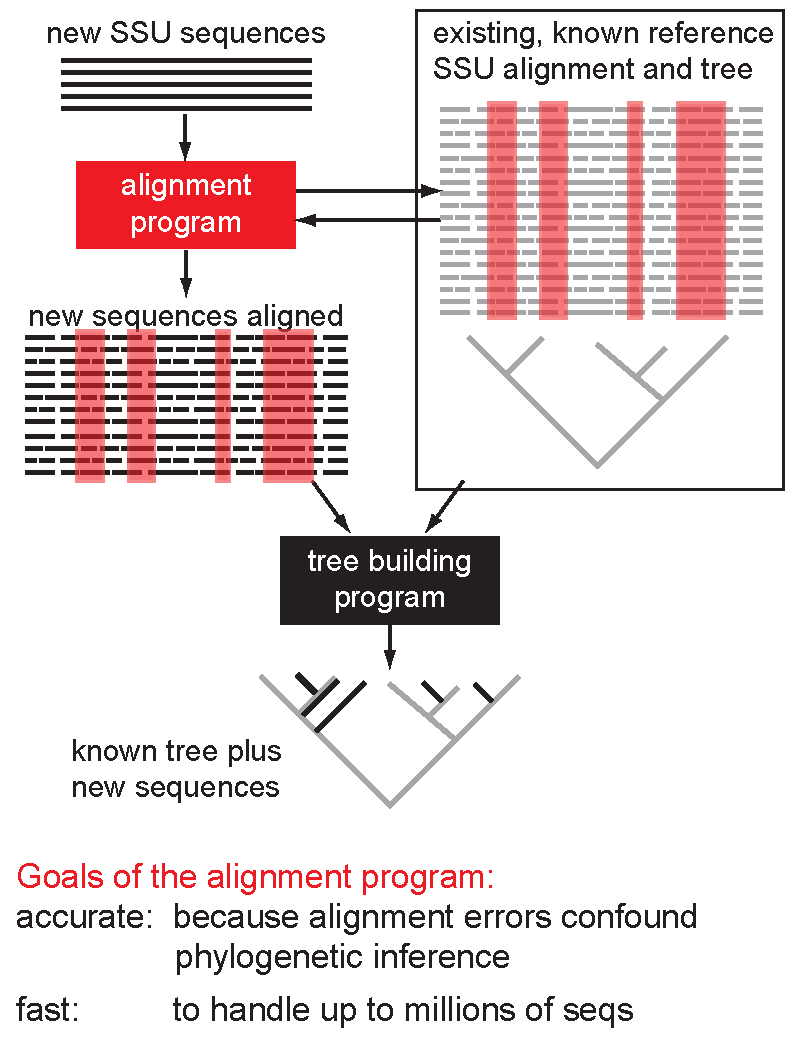
\includegraphics[height=7in]{figs/seq2tree-masked}}
\vfill
\end{slide}
%%%%%%%%%%%%%%%%%%%%%%%%%%%%%%%%%%%%%%%%%%%%%%%%%%%%%%%%%%%%%%%%%%%%%%%%%%
%%%%%%%%%%%%%%%%%%%%%%%%%%%%%%%%%%%%%%%%%%%%%%%%%%%%%%%%%%%%%%%%%%%%%%%%%
\begin{slide}
\begin{center}

\textbf{Phil Hugenholtz's manually created mask}
\end{center}
\small

\begin{center}
\includegraphics[height=7.5in]{figs/lmph-on-1513}

\end{center}
\vfill
\end{slide}
%%%%%%%%%%%%%%%%%%%%%%%%%%%%%%%%%%%%%%%%%%%%%%%%%%%%%%%%%%%%%%%%%%%%%%%%%%%%%%%%%%%%%%%%%%%%%
\begin{slide}\begin{center}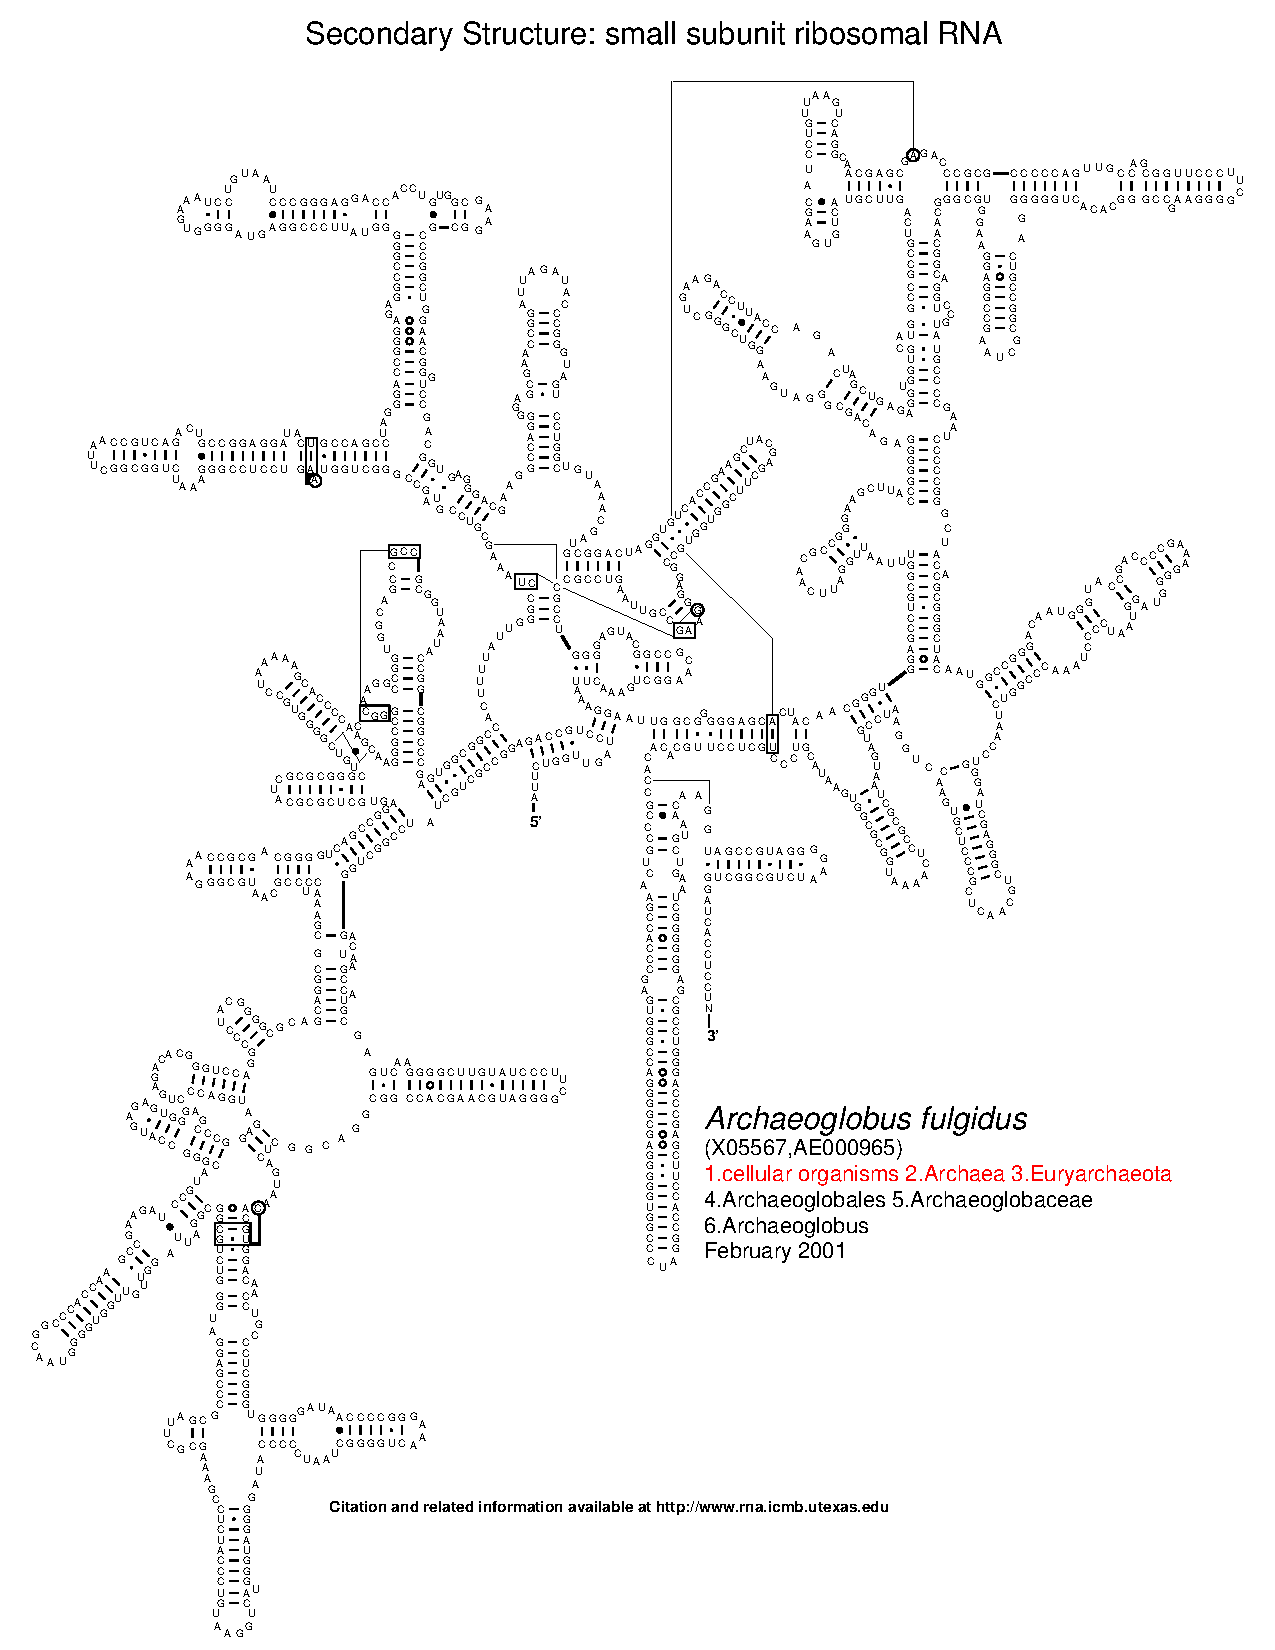
\includegraphics[height=8in]{figs/arc-1}\end{center}\vfill\end{slide}
%%%%%%%%%%%%%%%%%%%%%%%%%%%%%%%%%%%%%%%%%%%%%%%%%%%%%%%%%%%%%%%%%%%%%%%%%%%%%%%%%%%%%%%%%%%%%
\begin{slide}\begin{center}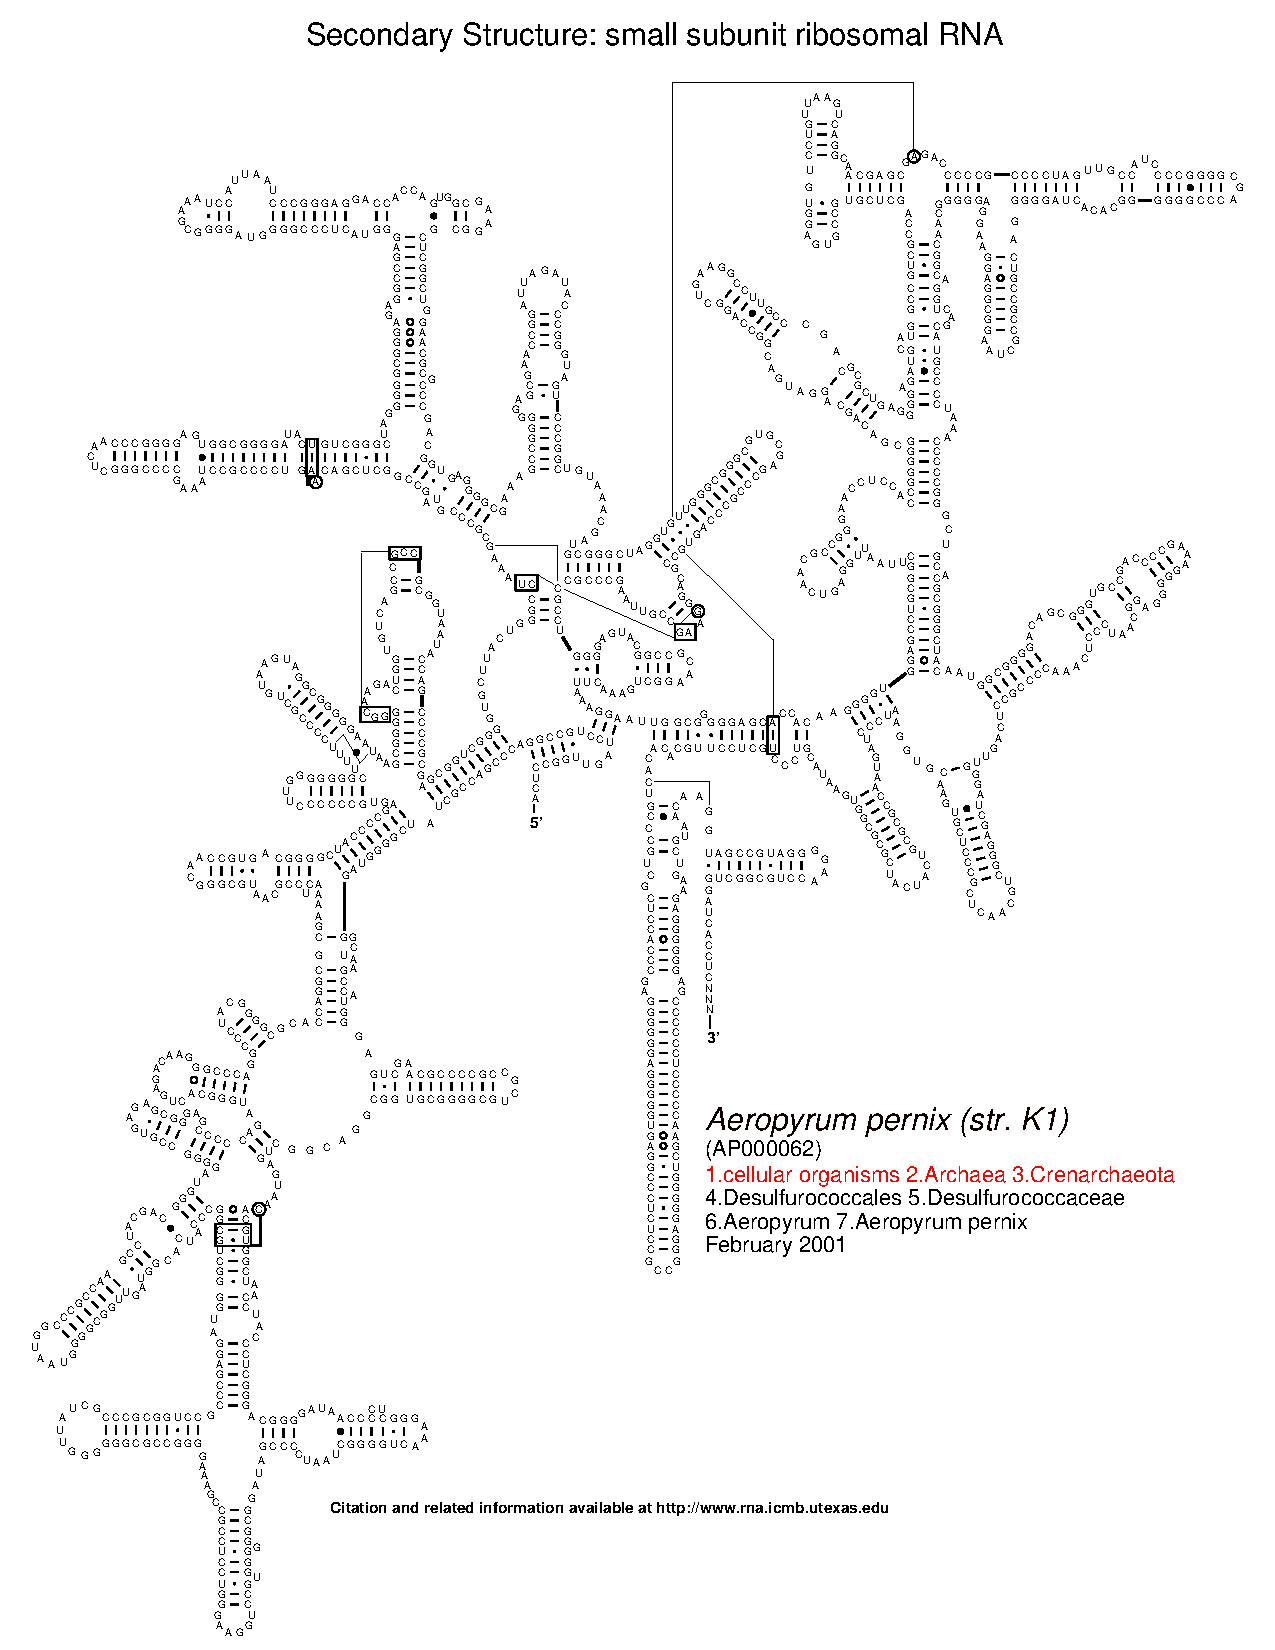
\includegraphics[height=8in]{figs/arc-2}\end{center}\vfill\end{slide}
%%%%%%%%%%%%%%%%%%%%%%%%%%%%%%%%%%%%%%%%%%%%%%%%%%%%%%%%%%%%%%%%%%%%%%%%%%%%%%%%%%%%%%%%%%%%%
\begin{slide}\begin{center}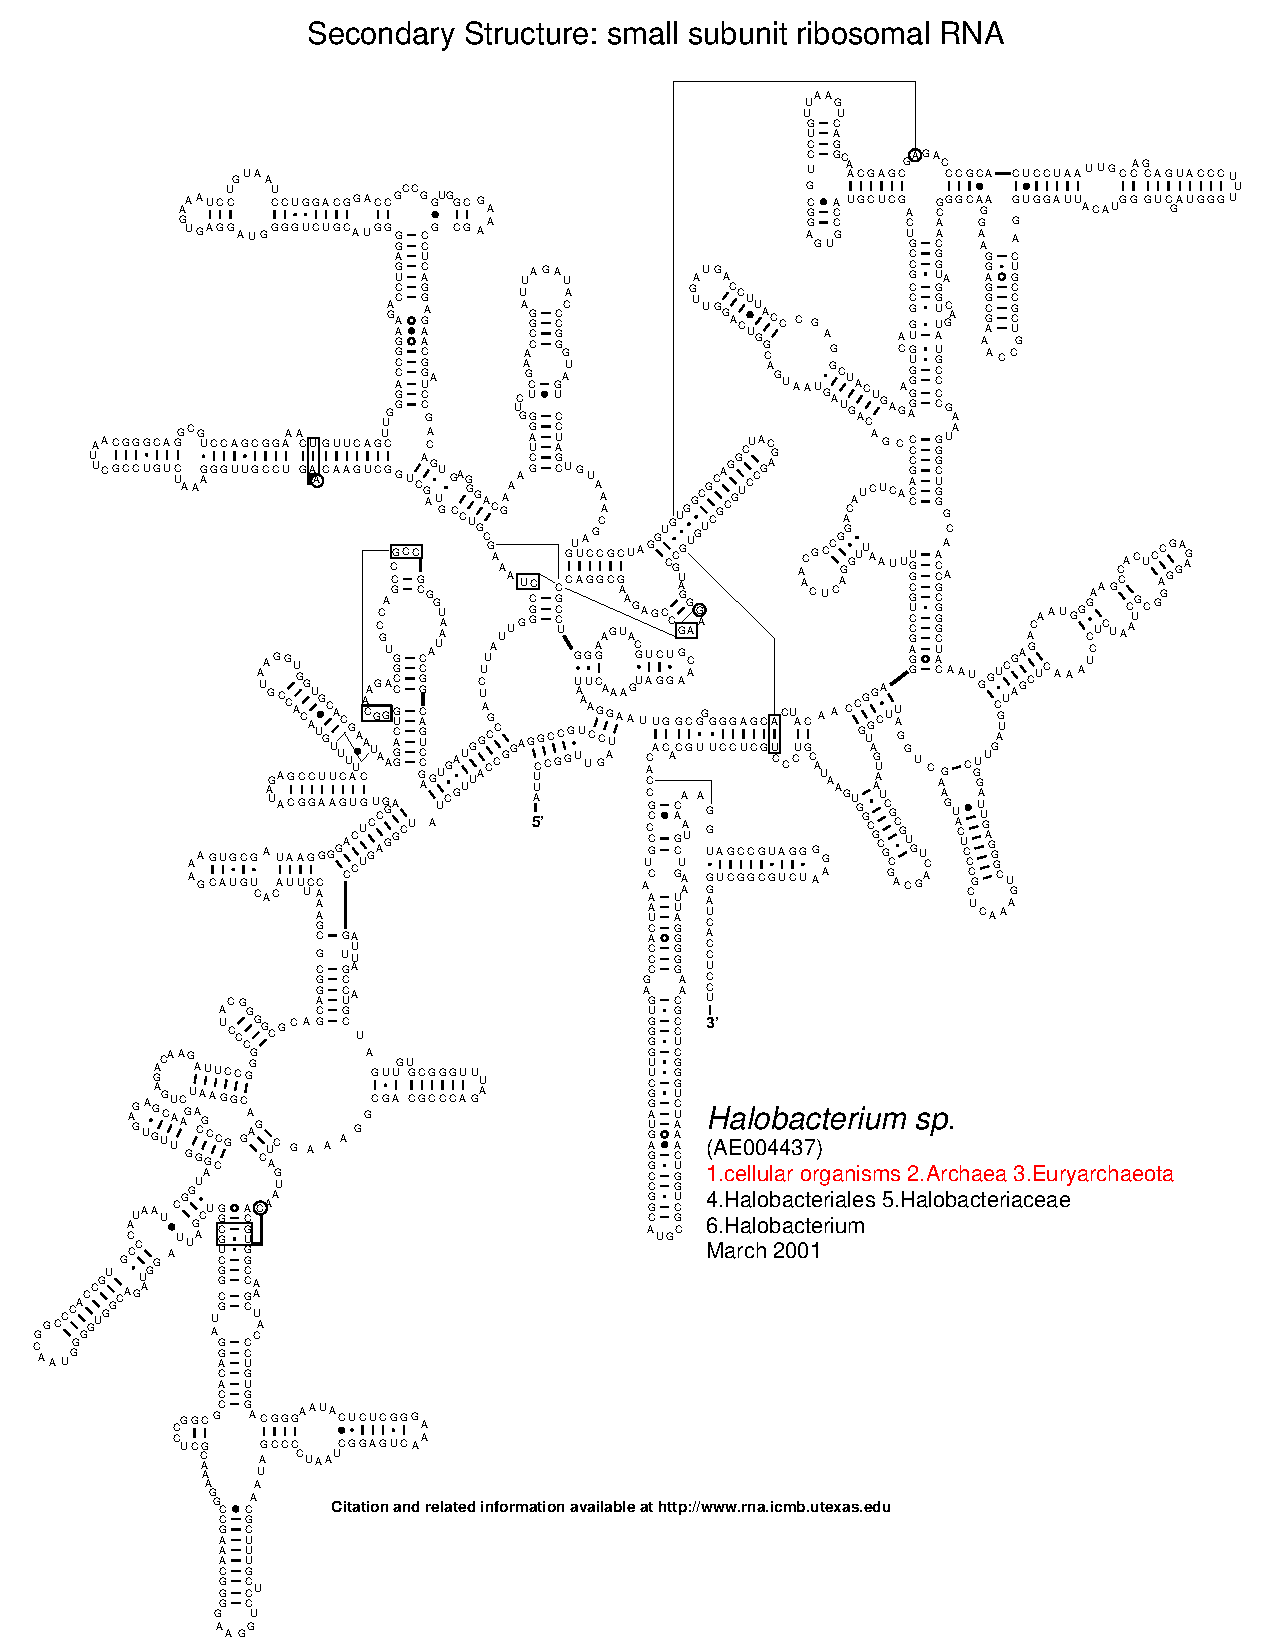
\includegraphics[height=8in]{figs/arc-3}\end{center}\vfill\end{slide}
%%%%%%%%%%%%%%%%%%%%%%%%%%%%%%%%%%%%%%%%%%%%%%%%%%%%%%%%%%%%%%%%%%%%%%%%%%%%%%%%%%%%%%%%%%%%%
%\begin{slide}\begin{center}\includegraphics[height=8in]{figs/arc-4}\end{center}\vfill\end{slide}
%%%%%%%%%%%%%%%%%%%%%%%%%%%%%%%%%%%%%%%%%%%%%%%%%%%%%%%%%%%%%%%%%%%%%%%%%%%%%%%%%%%%%%%%%%%%%
%\begin{slide}\begin{center}\includegraphics[height=8in]{figs/arc-5}\end{center}\vfill\end{slide}
%%%%%%%%%%%%%%%%%%%%%%%%%%%%%%%%%%%%%%%%%%%%%%%%%%%%%%%%%%%%%%%%%%%%%%%%%%%%%%%%%%%%%%%%%%%%%
%\begin{slide}\begin{center}\includegraphics[height=8in]{figs/arc-6}\end{center}\vfill\end{slide}
%%%%%%%%%%%%%%%%%%%%%%%%%%%%%%%%%%%%%%%%%%%%%%%%%%%%%%%%%%%%%%%%%%%%%%%%%%%%%%%%%%%%%%%%%%%%%
%\begin{slide}\begin{center}\includegraphics[height=8in]{figs/arc-7}\end{center}\vfill\end{slide}
%%%%%%%%%%%%%%%%%%%%%%%%%%%%%%%%%%%%%%%%%%%%%%%%%%%%%%%%%%%%%%%%%%%%%%%%%%%%%%%%%%%%%%%%%%%%%
%\begin{slide}\begin{center}\includegraphics[height=8in]{figs/arc-8}\end{center}\vfill\end{slide}
%%%%%%%%%%%%%%%%%%%%%%%%%%%%%%%%%%%%%%%%%%%%%%%%%%%%%%%%%%%%%%%%%%%%%%%%%%%%%%%%%%%%%%%%%%%%%
%\begin{slide}\begin{center}\includegraphics[height=8in]{figs/arc-9}\end{center}\vfill\end{slide}
%%%%%%%%%%%%%%%%%%%%%%%%%%%%%%%%%%%%%%%%%%%%%%%%%%%%%%%%%%%%%%%%%%%%%%%%%%%%%%%%%%%%%%%%%%%%%
%\begin{slide}\begin{center}\includegraphics[height=8in]{figs/arc-10}\end{center}\vfill\end{slide}
%%%%%%%%%%%%%%%%%%%%%%%%%%%%%%%%%%%%%%%%%%%%%%%%%%%%%%%%%%%%%%%%%%%%%%%%%%%%%%%%%%%%%%%%%%%%%
\begin{slide}\begin{center}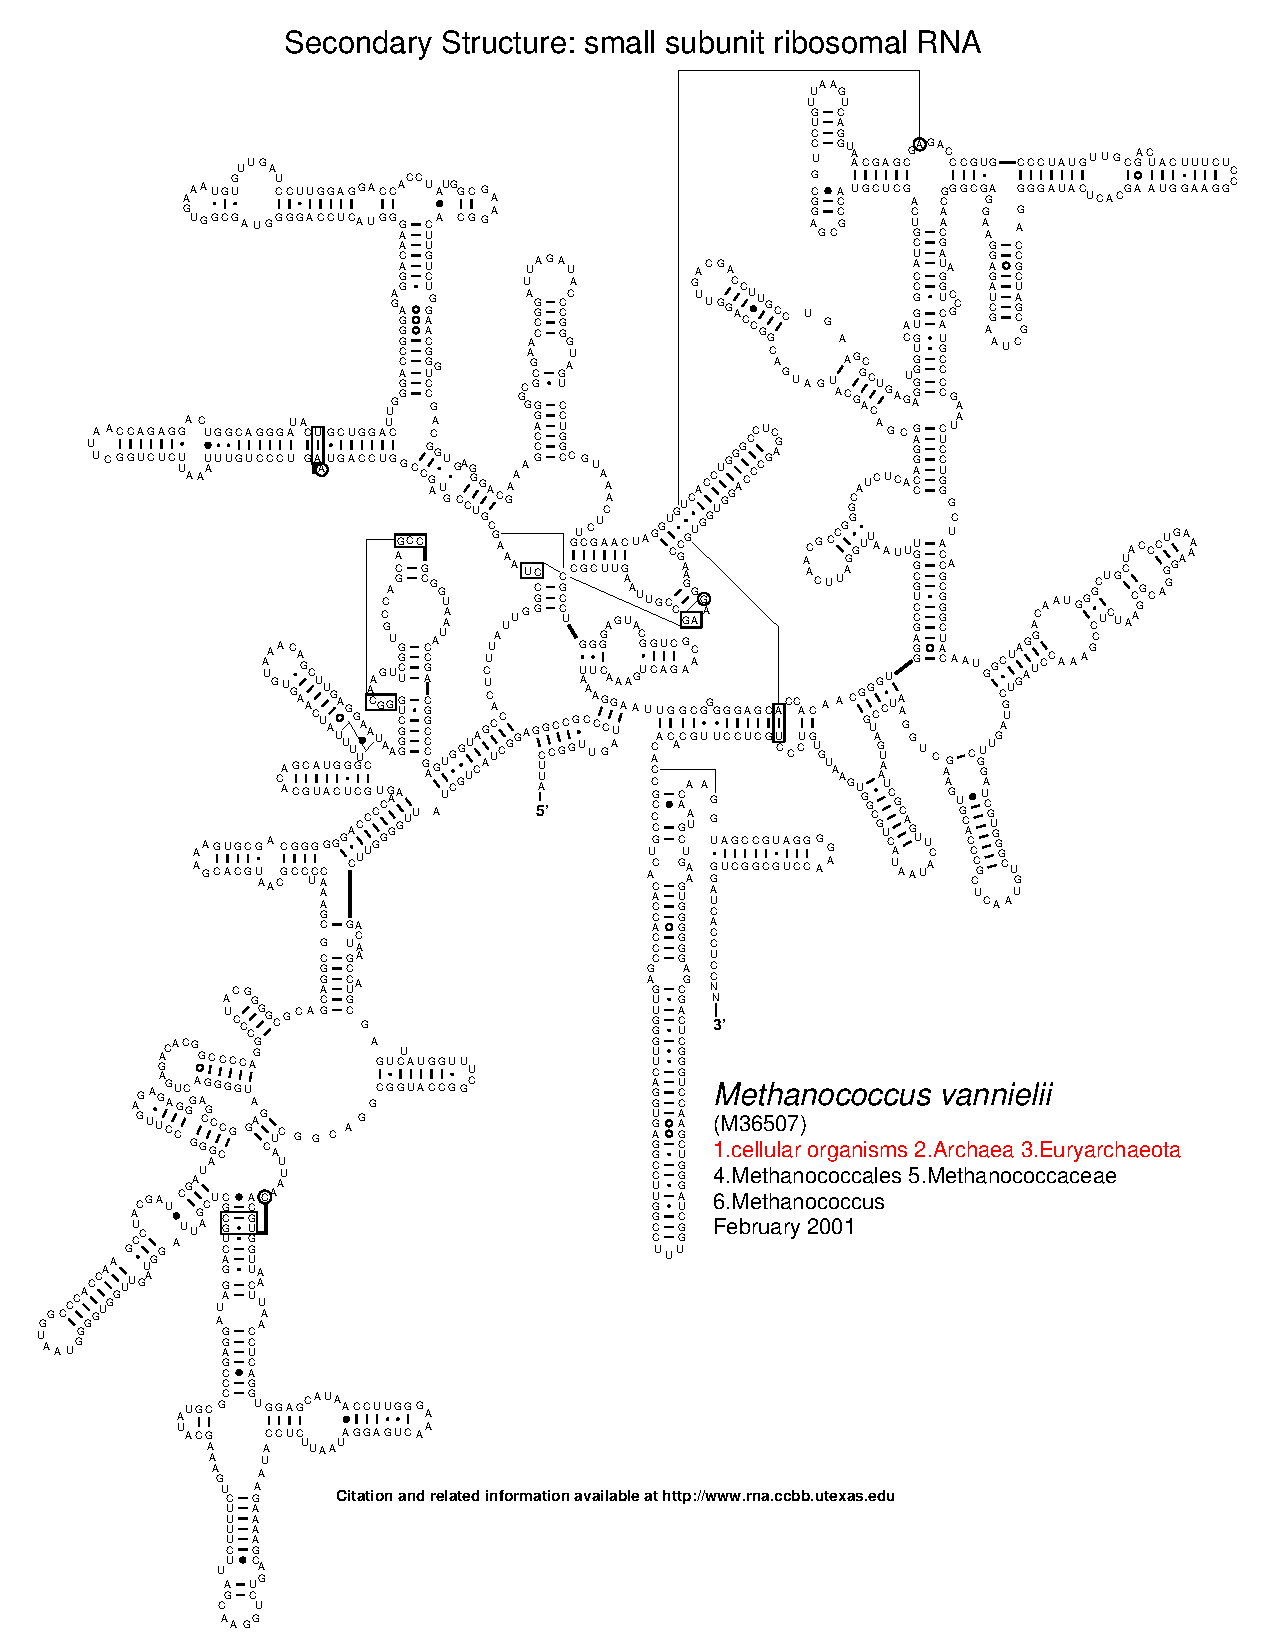
\includegraphics[height=8in]{figs/arc-11}\end{center}\vfill\end{slide}
%%%%%%%%%%%%%%%%%%%%%%%%%%%%%%%%%%%%%%%%%%%%%%%%%%%%%%%%%%%%%%%%%%%%%%%%%%%%%%%%%%%%%%%%%%%%%
\begin{slide}\begin{center}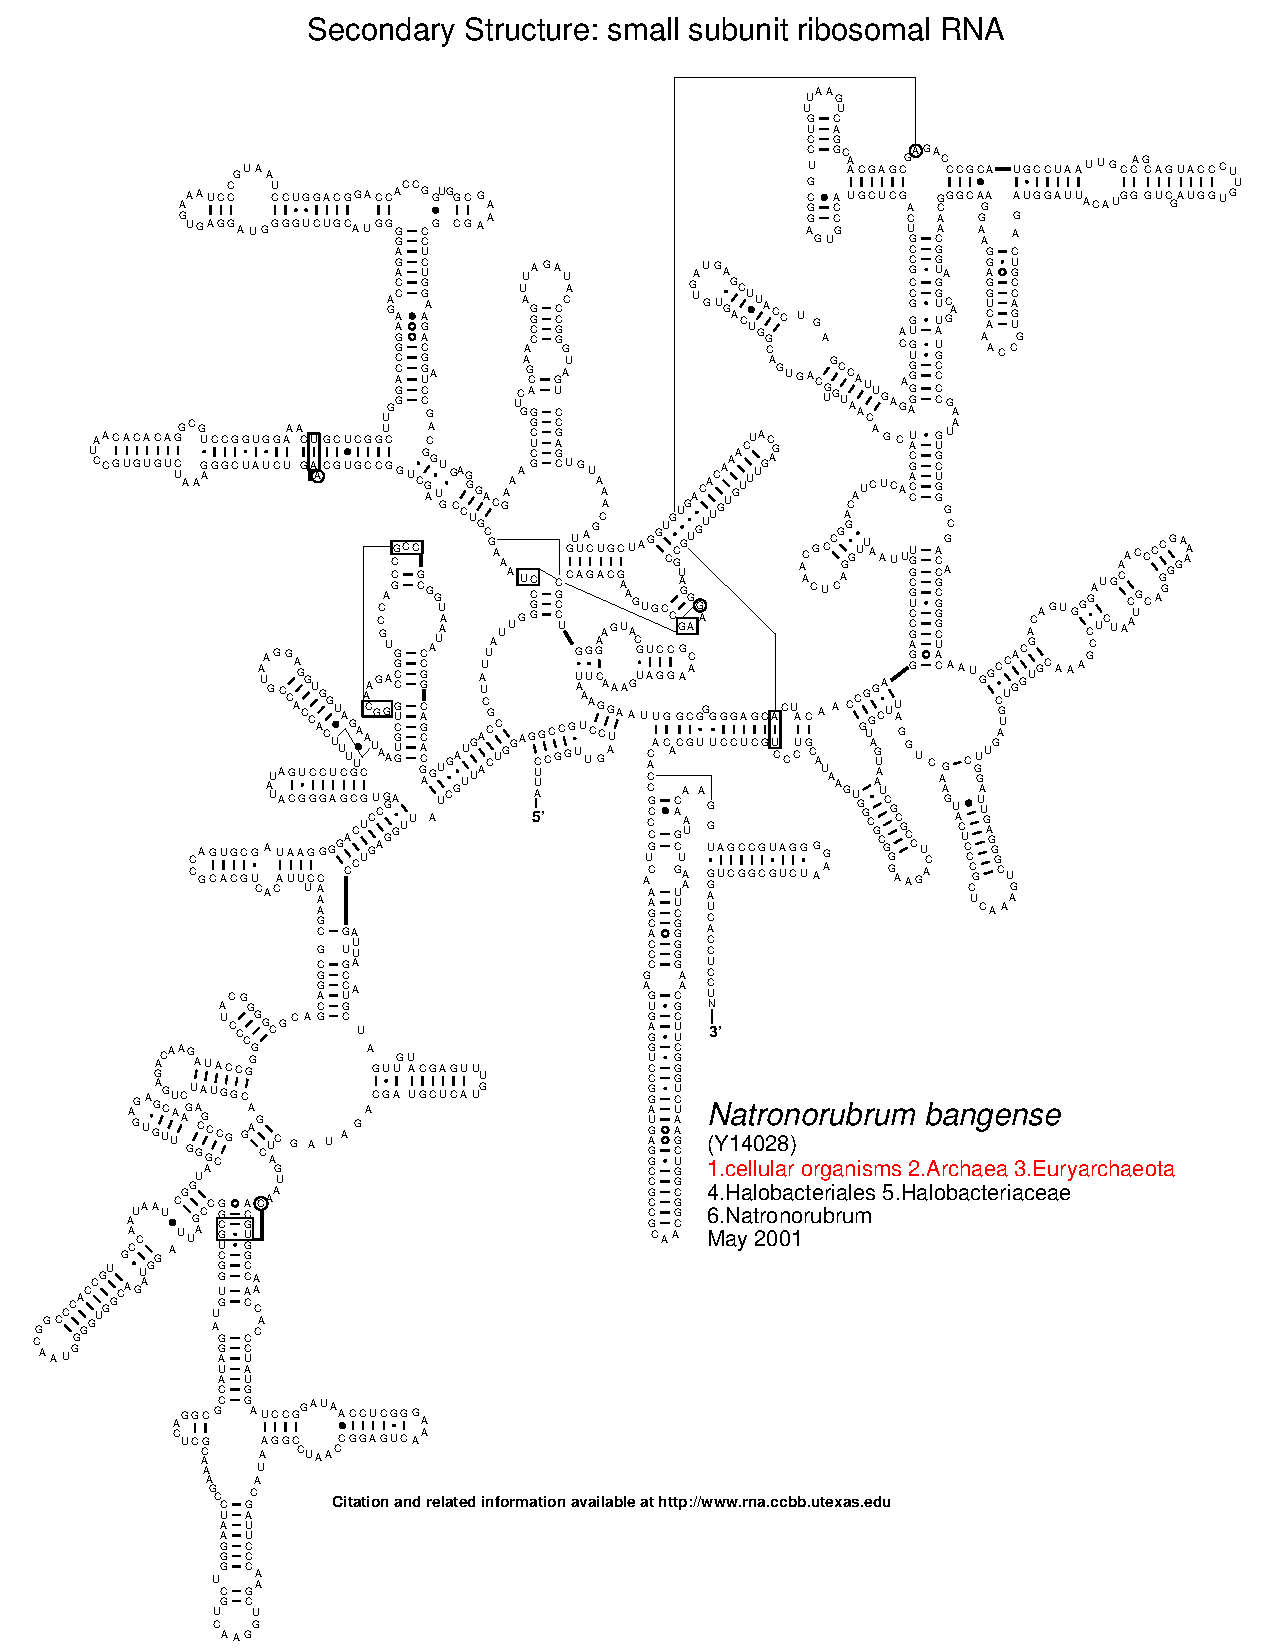
\includegraphics[height=8in]{figs/arc-12}\end{center}\vfill\end{slide}
%%%%%%%%%%%%%%%%%%%%%%%%%%%%%%%%%%%%%%%%%%%%%%%%%%%%%%%%%%%%%%%%%%%%%%%%%%%%%%%%%%%%%%%%%%%%%
\begin{slide}\begin{center}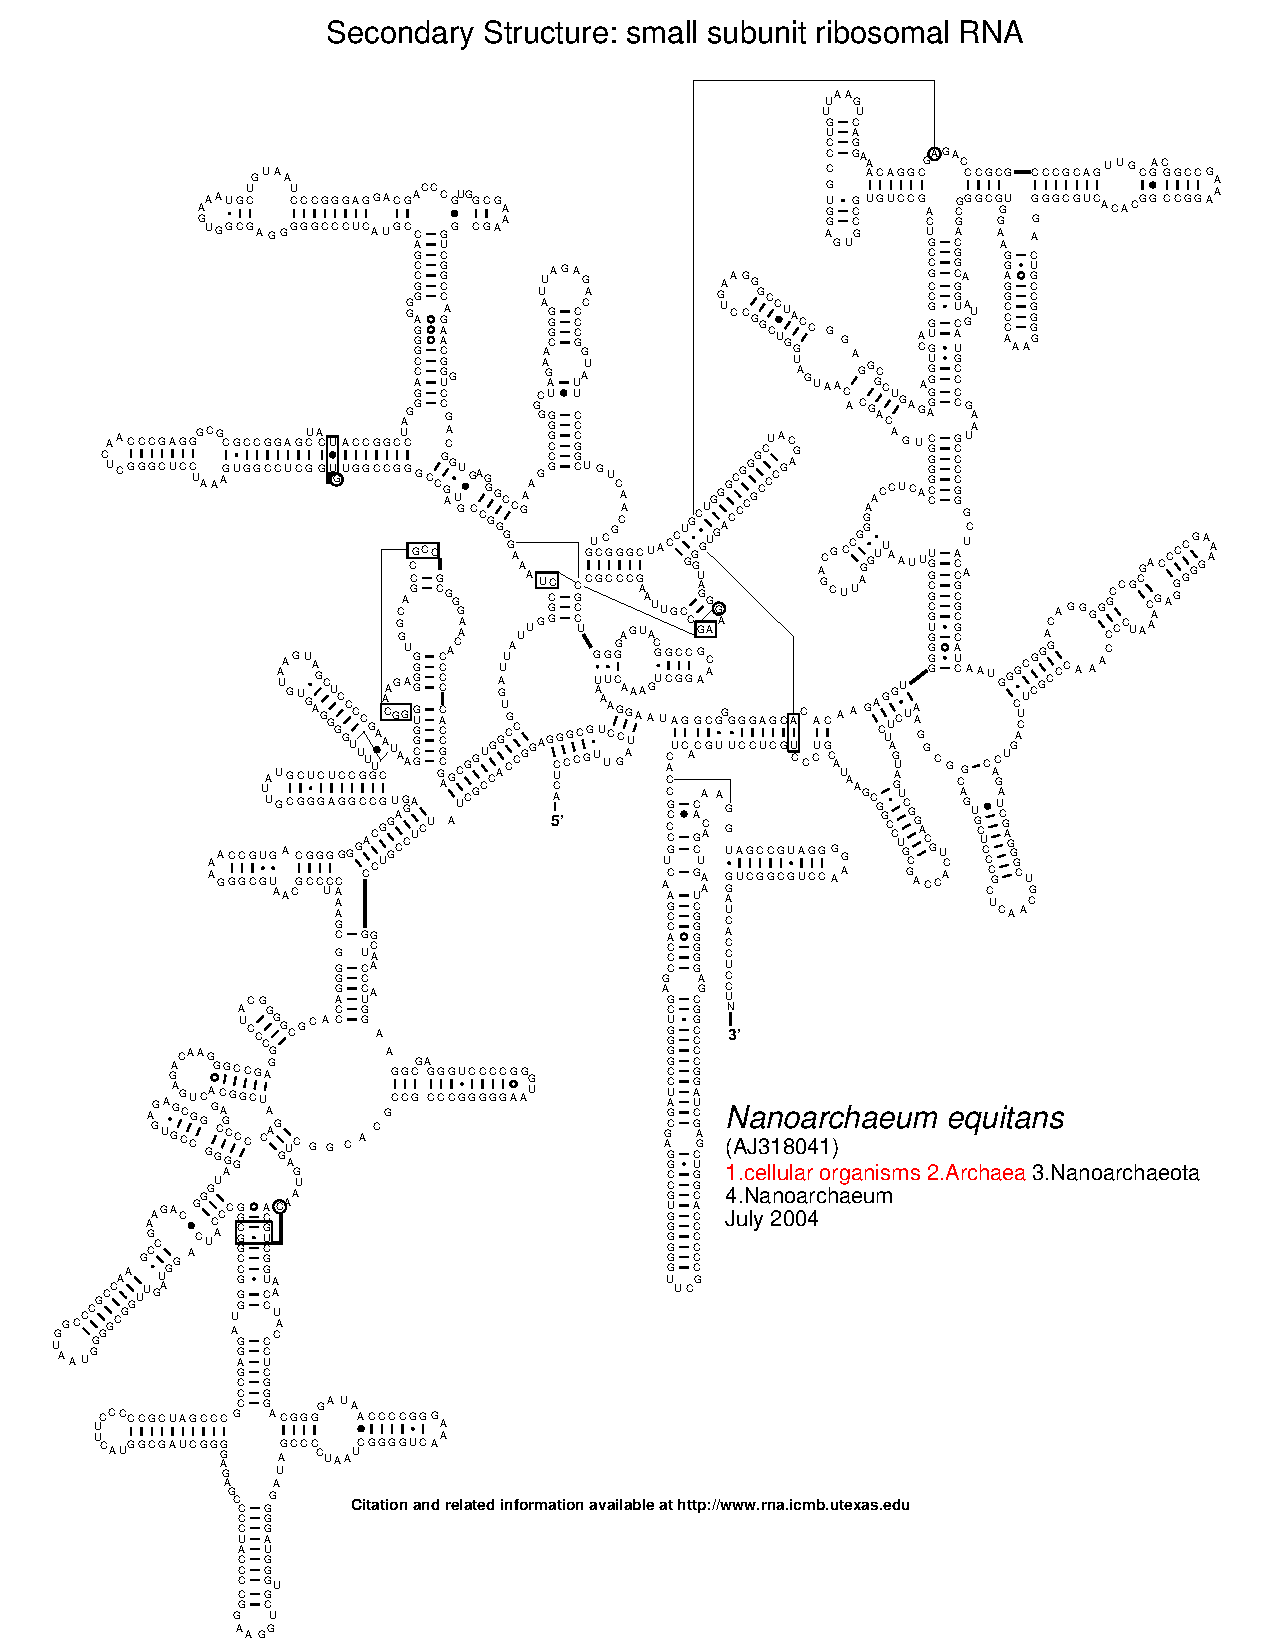
\includegraphics[height=8in]{figs/arc-13}\end{center}\vfill\end{slide}
%%%%%%%%%%%%%%%%%%%%%%%%%%%%%%%%%%%%%%%%%%%%%%%%%%%%%%%%%%%%%%%%%%%%%%%%%%%%%%%%%%%%%%%%%%%%%
\begin{slide}\begin{center}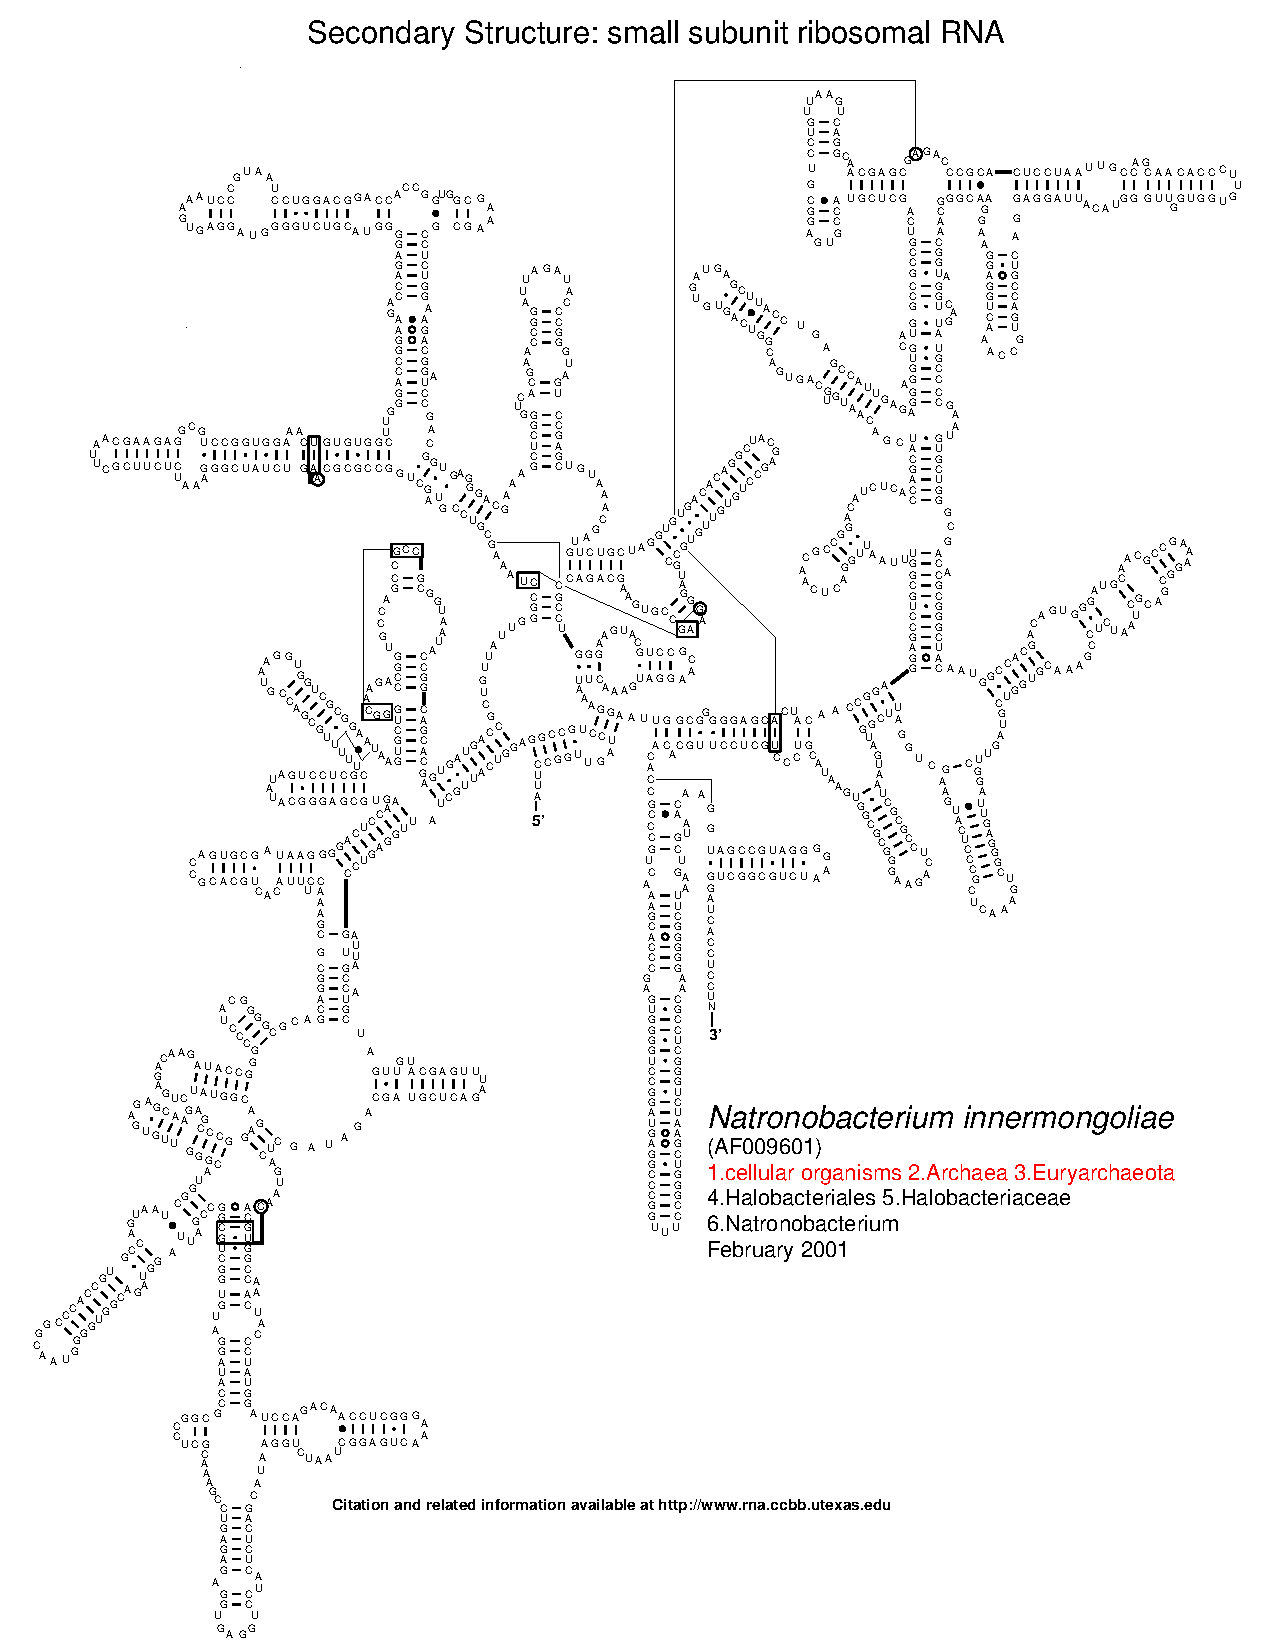
\includegraphics[height=8in]{figs/arc-14}\end{center}\vfill\end{slide}
%%%%%%%%%%%%%%%%%%%%%%%%%%%%%%%%%%%%%%%%%%%%%%%%%%%%%%%%%%%%%%%%%%%%%%%%%%%%%%%%%%%%%%%%%%%%%
\begin{slide}\begin{center}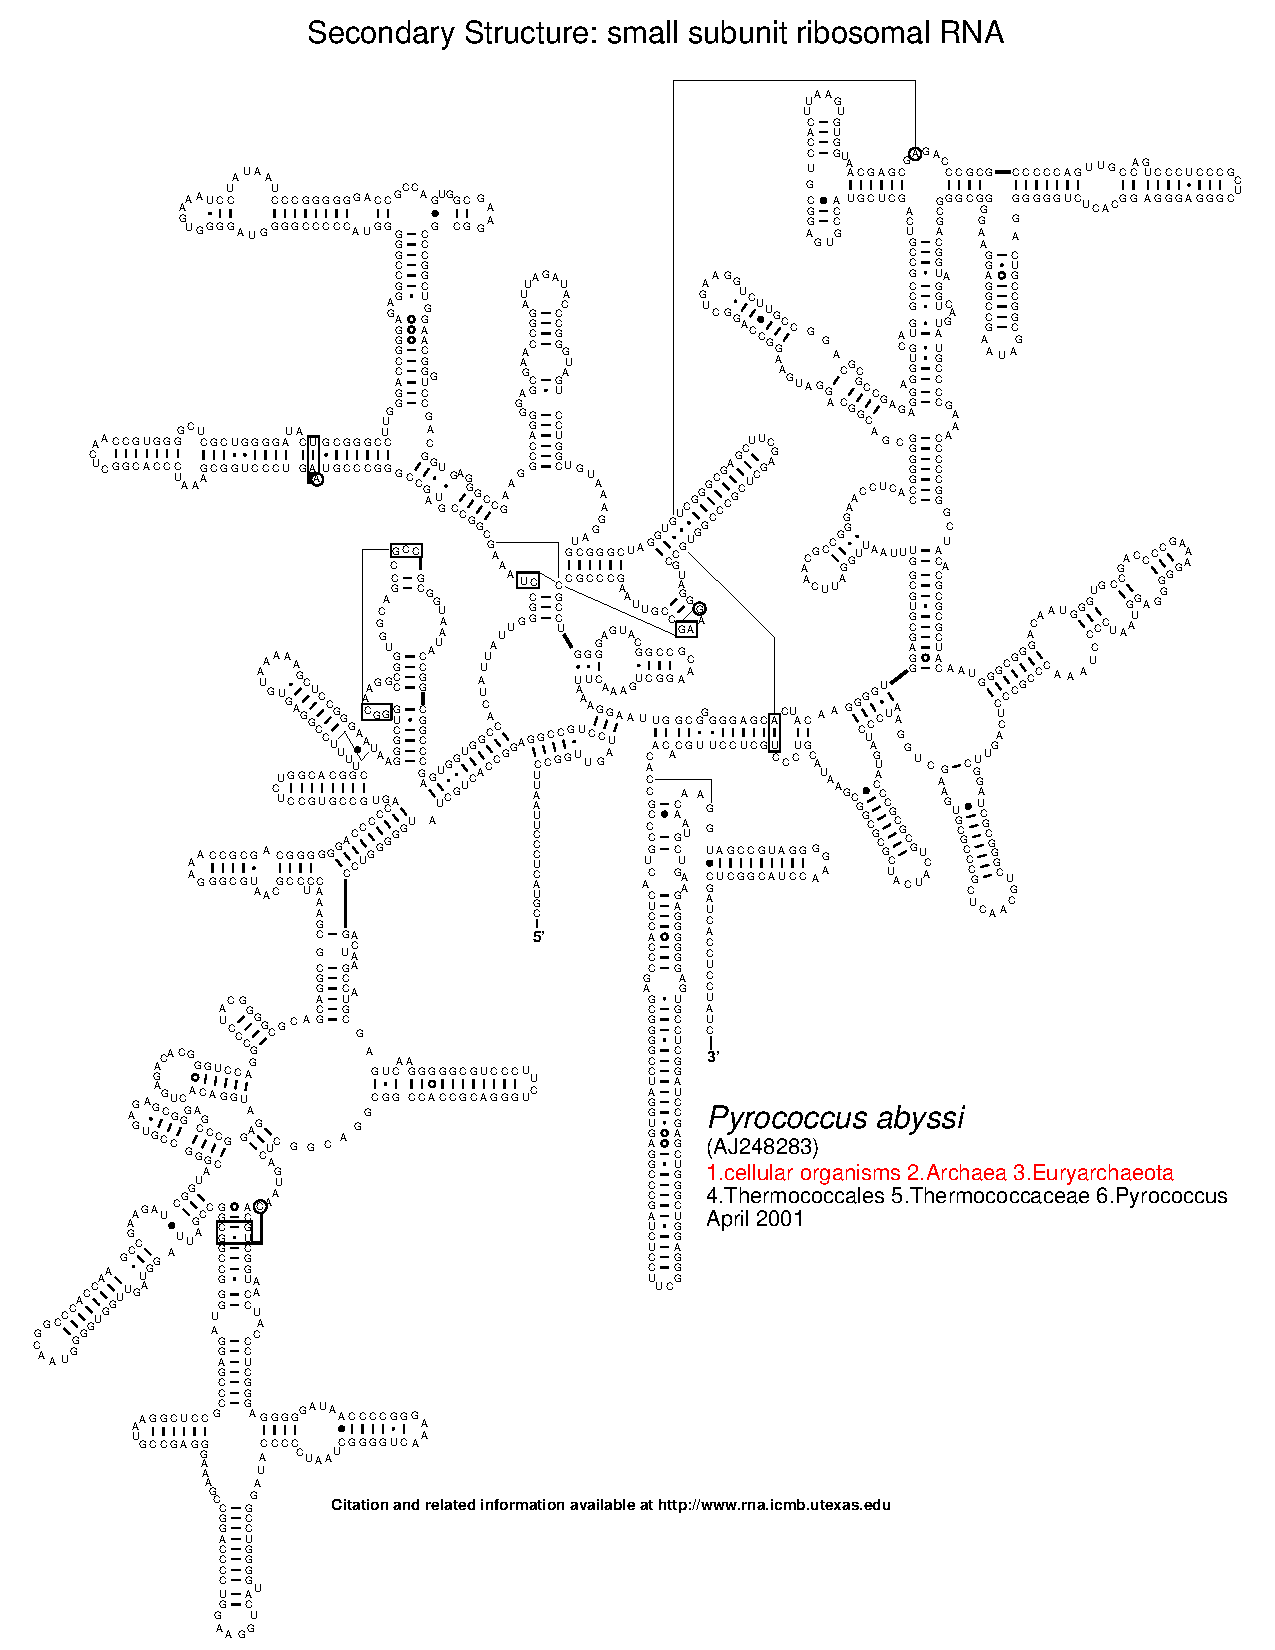
\includegraphics[height=8in]{figs/arc-15}\end{center}\vfill\end{slide}
%%%%%%%%%%%%%%%%%%%%%%%%%%%%%%%%%%%%%%%%%%%%%%%%%%%%%%%%%%%%%%%%%%%%%%%%%%%%%%%%%%%%%%%%%%%%%
\begin{slide}\begin{center}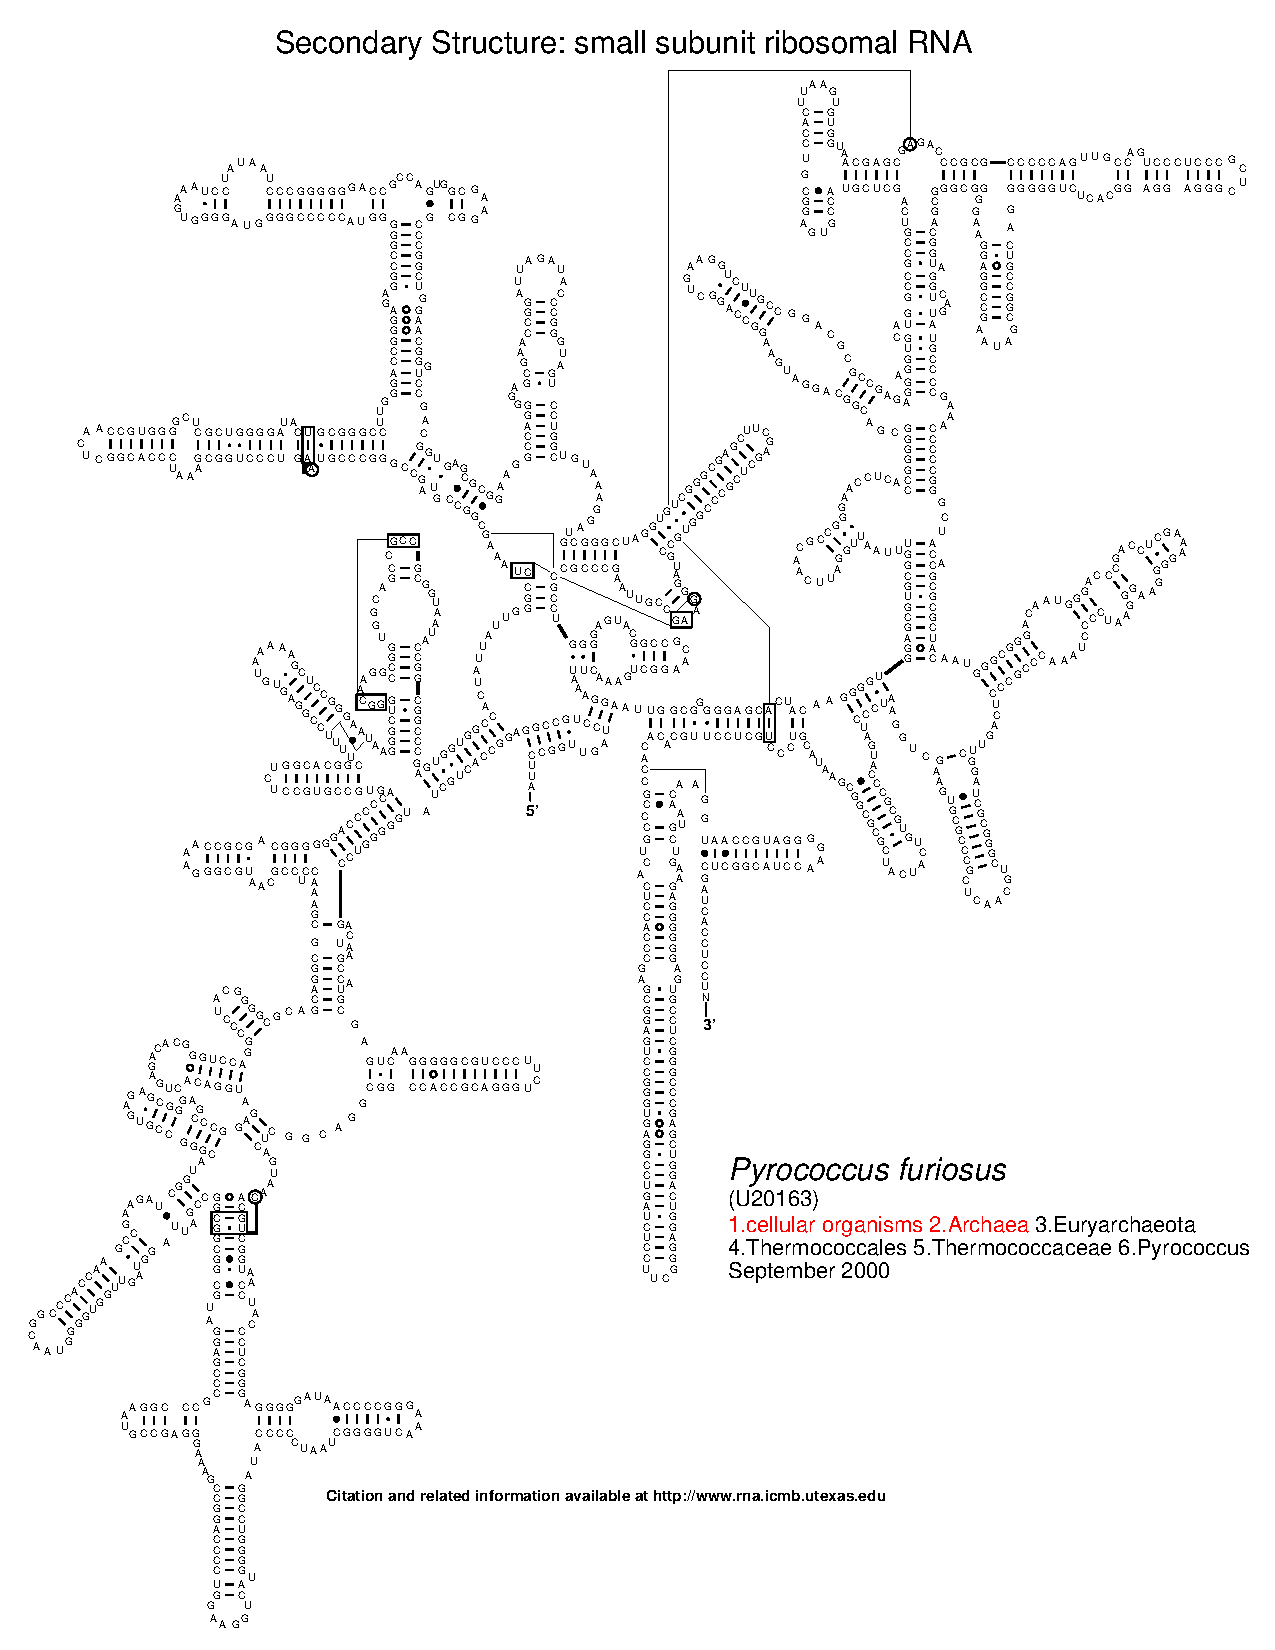
\includegraphics[height=8in]{figs/arc-16}\end{center}\vfill\end{slide}
%%%%%%%%%%%%%%%%%%%%%%%%%%%%%%%%%%%%%%%%%%%%%%%%%%%%%%%%%%%%%%%%%%%%%%%%%%%%%%%%%%%%%%%%%%%%%
\begin{slide}\begin{center}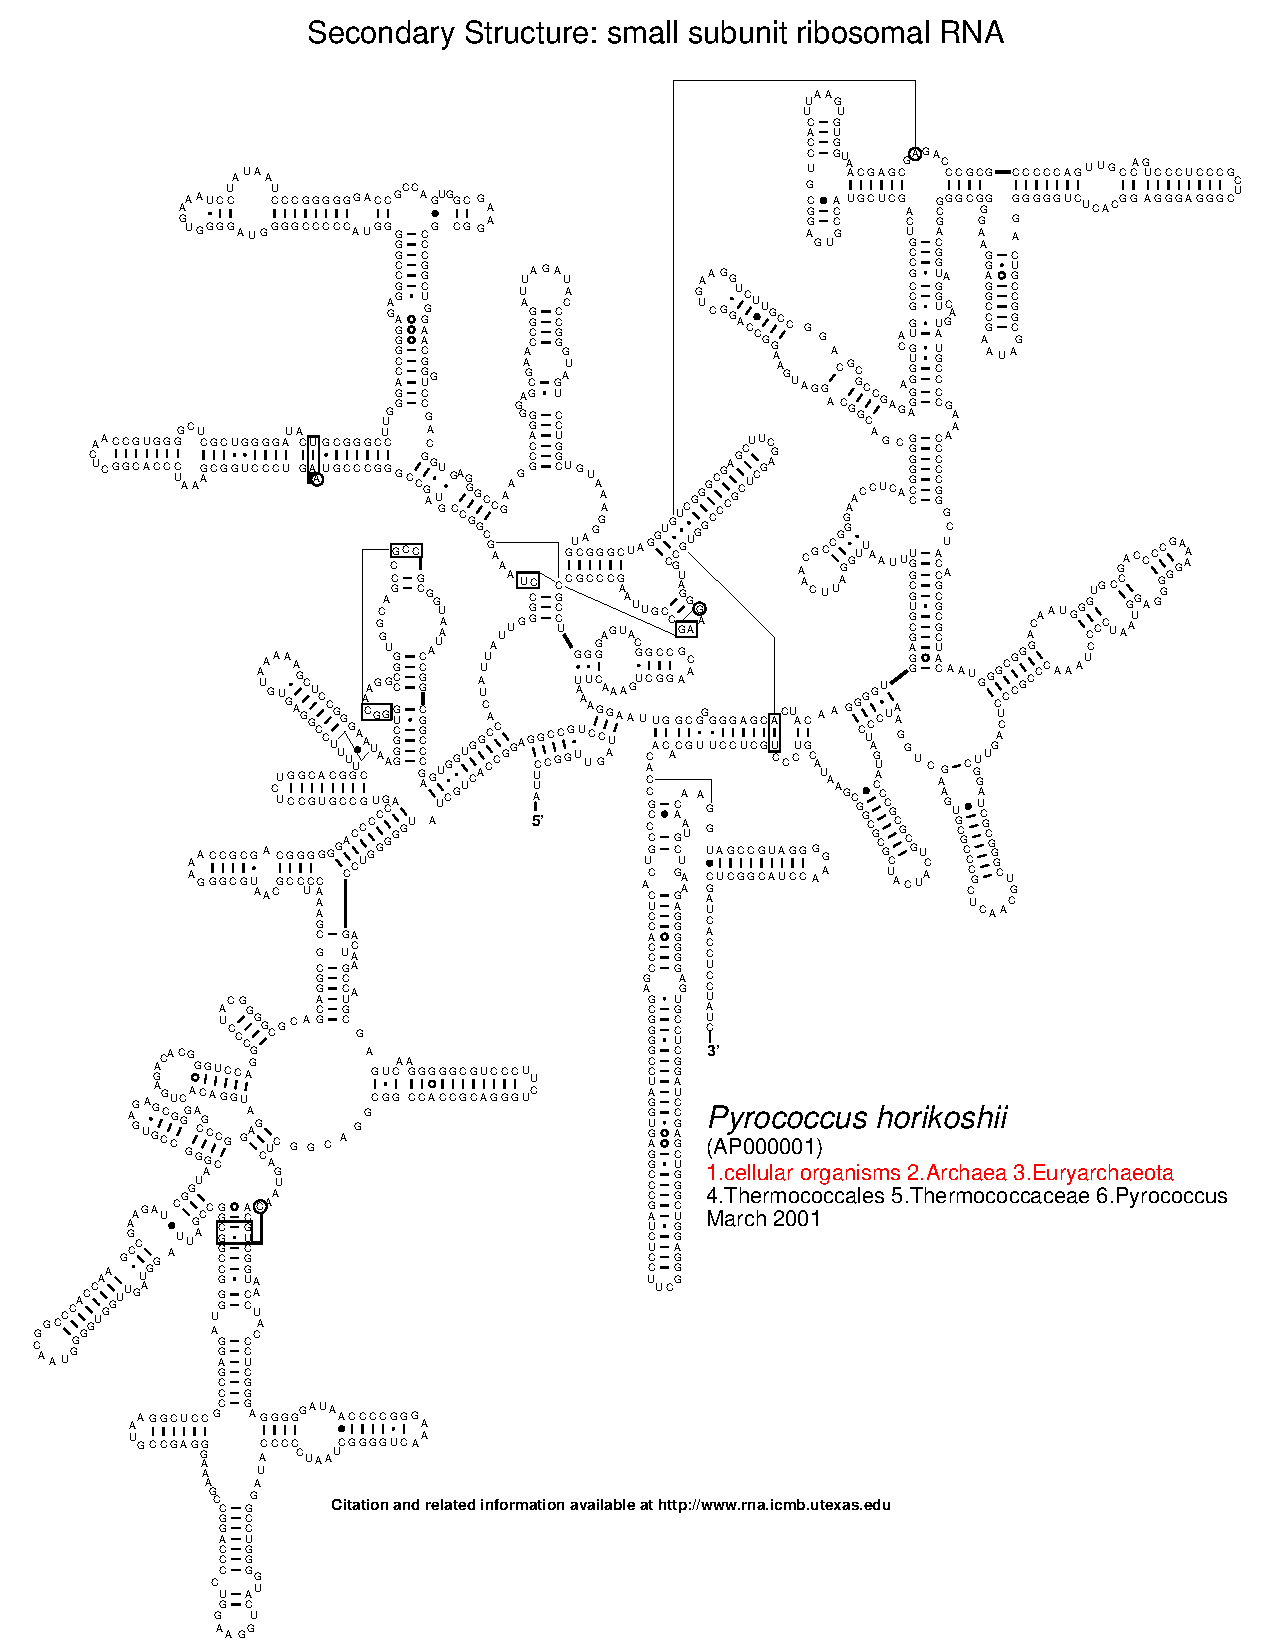
\includegraphics[height=8in]{figs/arc-17}\end{center}\vfill\end{slide}
%%%%%%%%%%%%%%%%%%%%%%%%%%%%%%%%%%%%%%%%%%%%%%%%%%%%%%%%%%%%%%%%%%%%%%%%%%%%%%%%%%%%%%%%%%%%%
\begin{slide}\begin{center}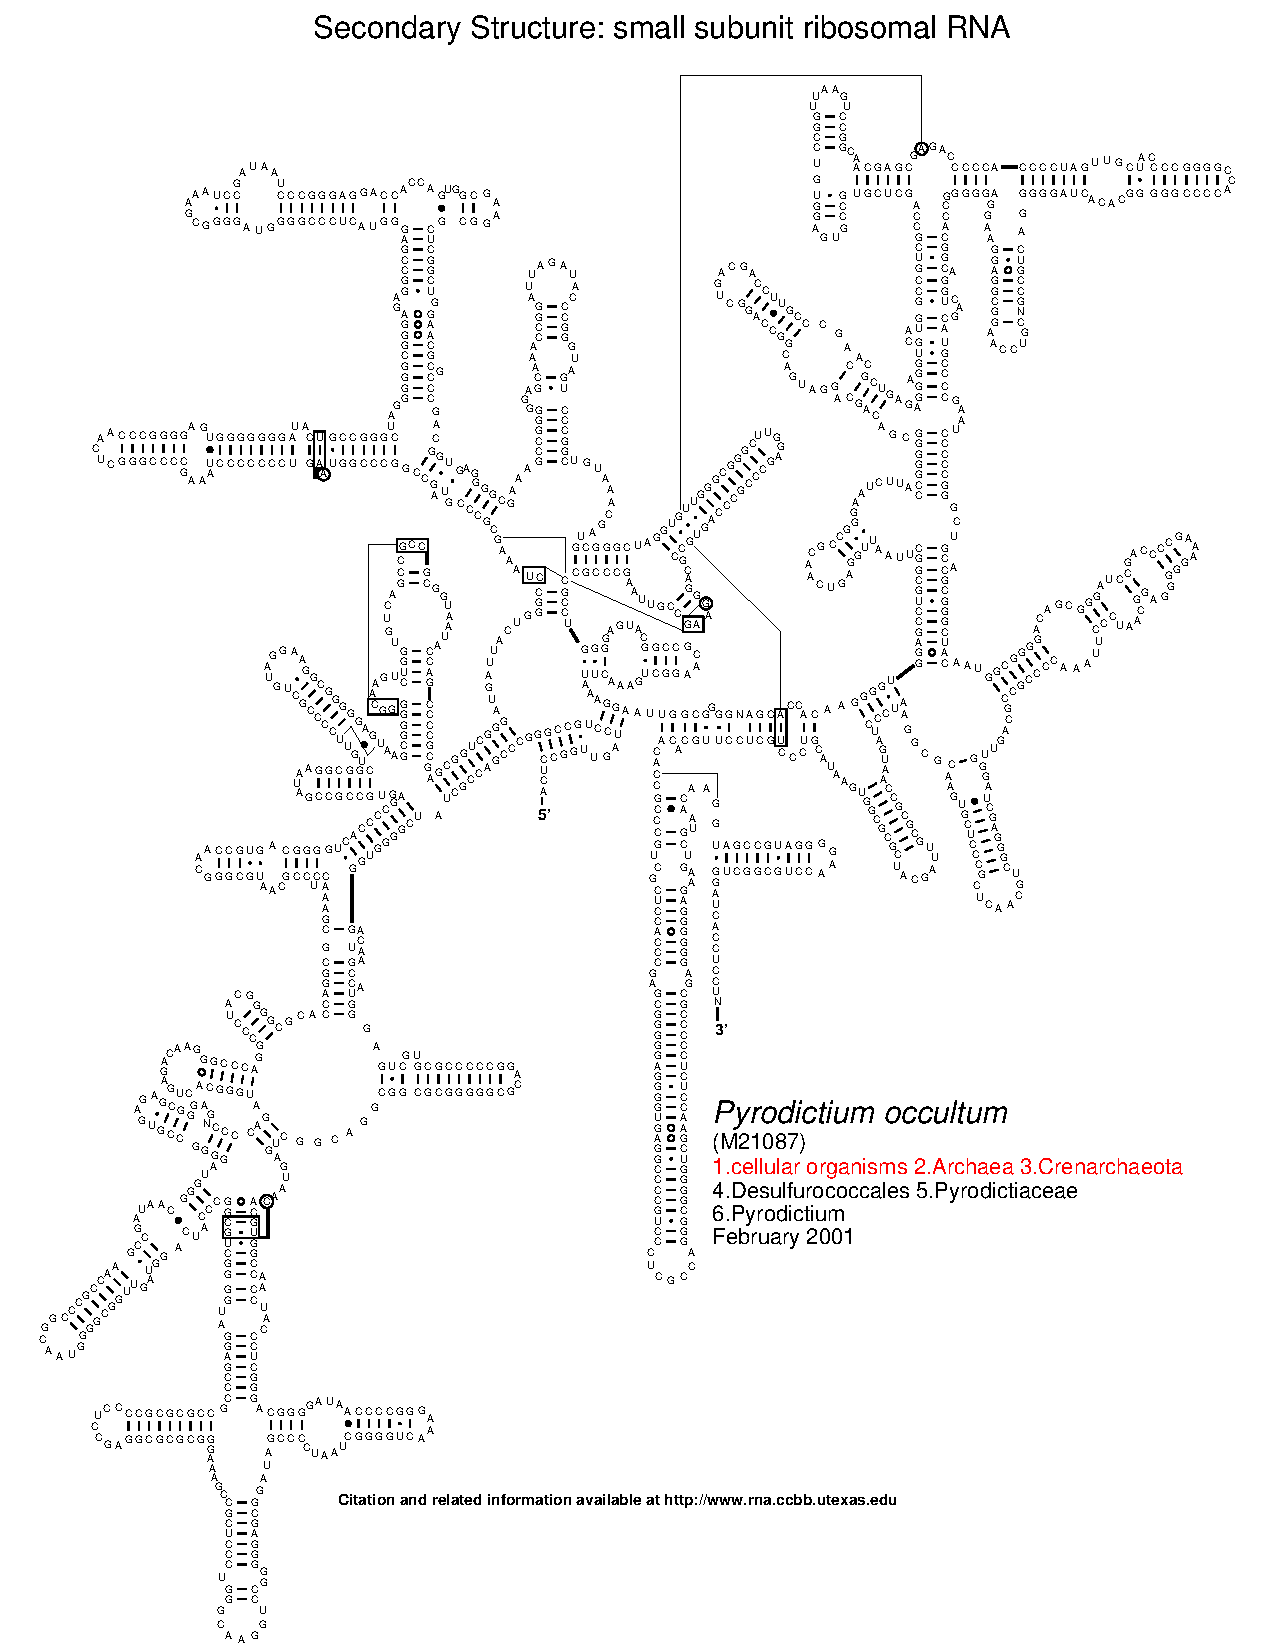
\includegraphics[height=8in]{figs/arc-18}\end{center}\vfill\end{slide}
%%%%%%%%%%%%%%%%%%%%%%%%%%%%%%%%%%%%%%%%%%%%%%%%%%%%%%%%%%%%%%%%%%%%%%%%%%%%%%%%%%%%%%%%%%%%%
\begin{slide}\begin{center}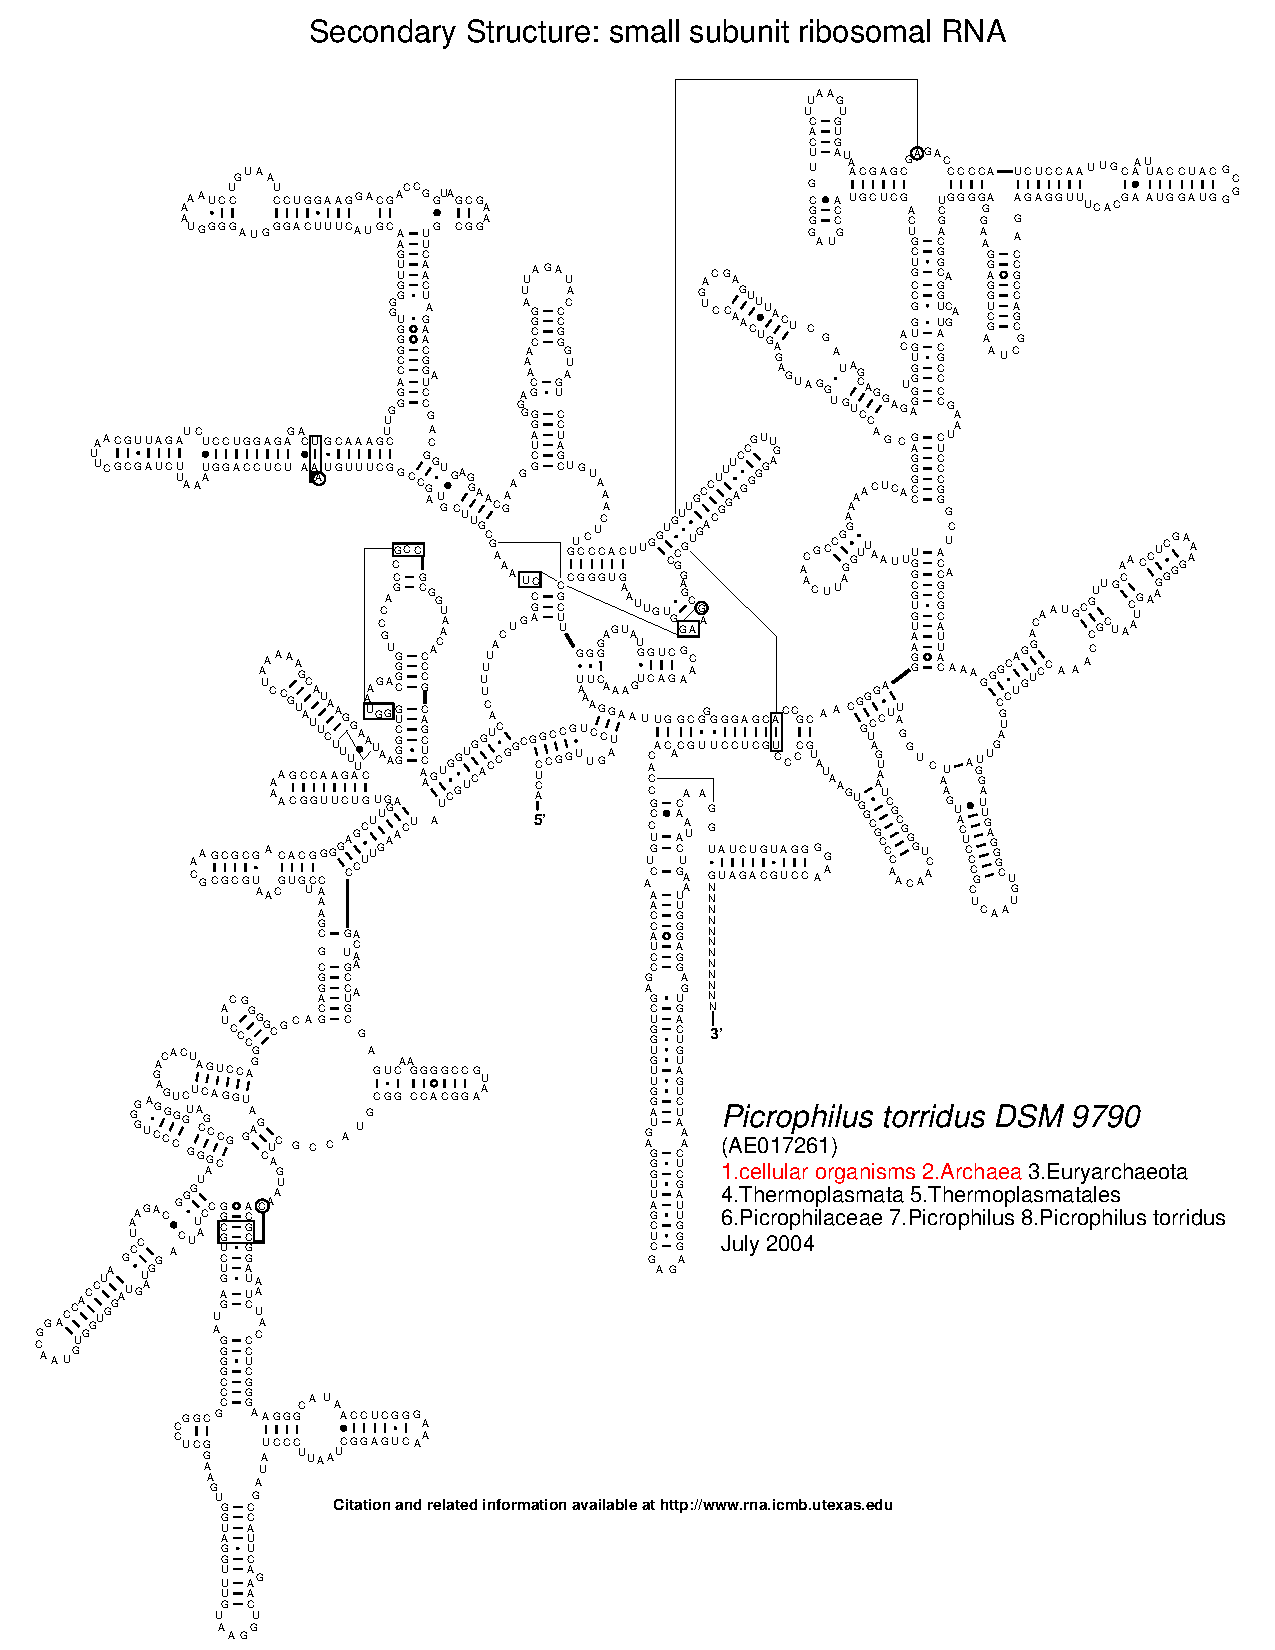
\includegraphics[height=8in]{figs/arc-19}\end{center}\vfill\end{slide}
%%%%%%%%%%%%%%%%%%%%%%%%%%%%%%%%%%%%%%%%%%%%%%%%%%%%%%%%%%%%%%%%%%%%%%%%%%%%%%%%%%%%%%%%%%%%%
%\begin{slide}\begin{center}\includegraphics[height=8in]{figs/arc-20}\end{center}\vfill\end{slide}
%%%%%%%%%%%%%%%%%%%%%%%%%%%%%%%%%%%%%%%%%%%%%%%%%%%%%%%%%%%%%%%%%%%%%%%%%%%%%%%%%%%%%%%%%%%%%
%\begin{slide}\begin{center}\includegraphics[height=8in]{figs/arc-21}\end{center}\vfill\end{slide}
%%%%%%%%%%%%%%%%%%%%%%%%%%%%%%%%%%%%%%%%%%%%%%%%%%%%%%%%%%%%%%%%%%%%%%%%%%%%%%%%%%%%%%%%%%%%%
\begin{slide}\begin{center}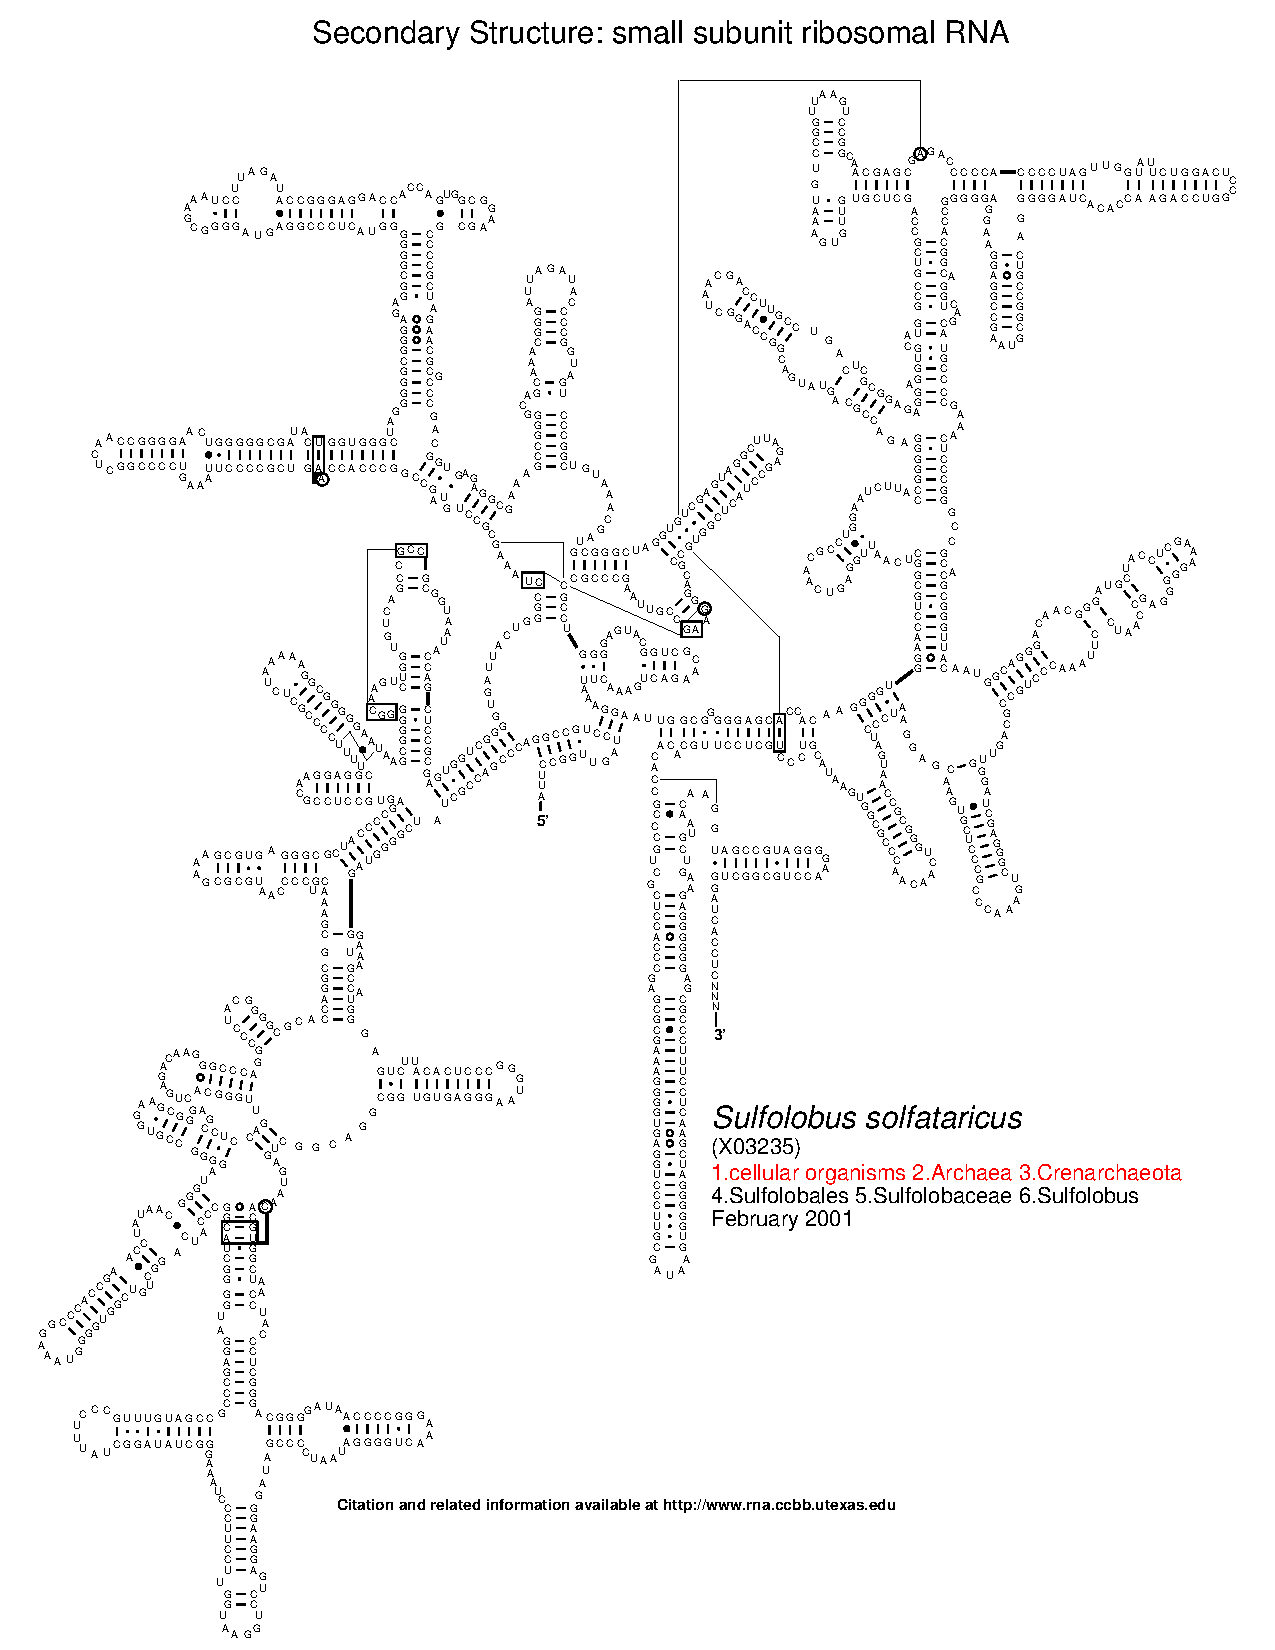
\includegraphics[height=8in]{figs/arc-22}\end{center}\vfill\end{slide}
%%%%%%%%%%%%%%%%%%%%%%%%%%%%%%%%%%%%%%%%%%%%%%%%%%%%%%%%%%%%%%%%%%%%%%%%%%%%%%%%%%%%%%%%%%%%%
\begin{slide}\begin{center}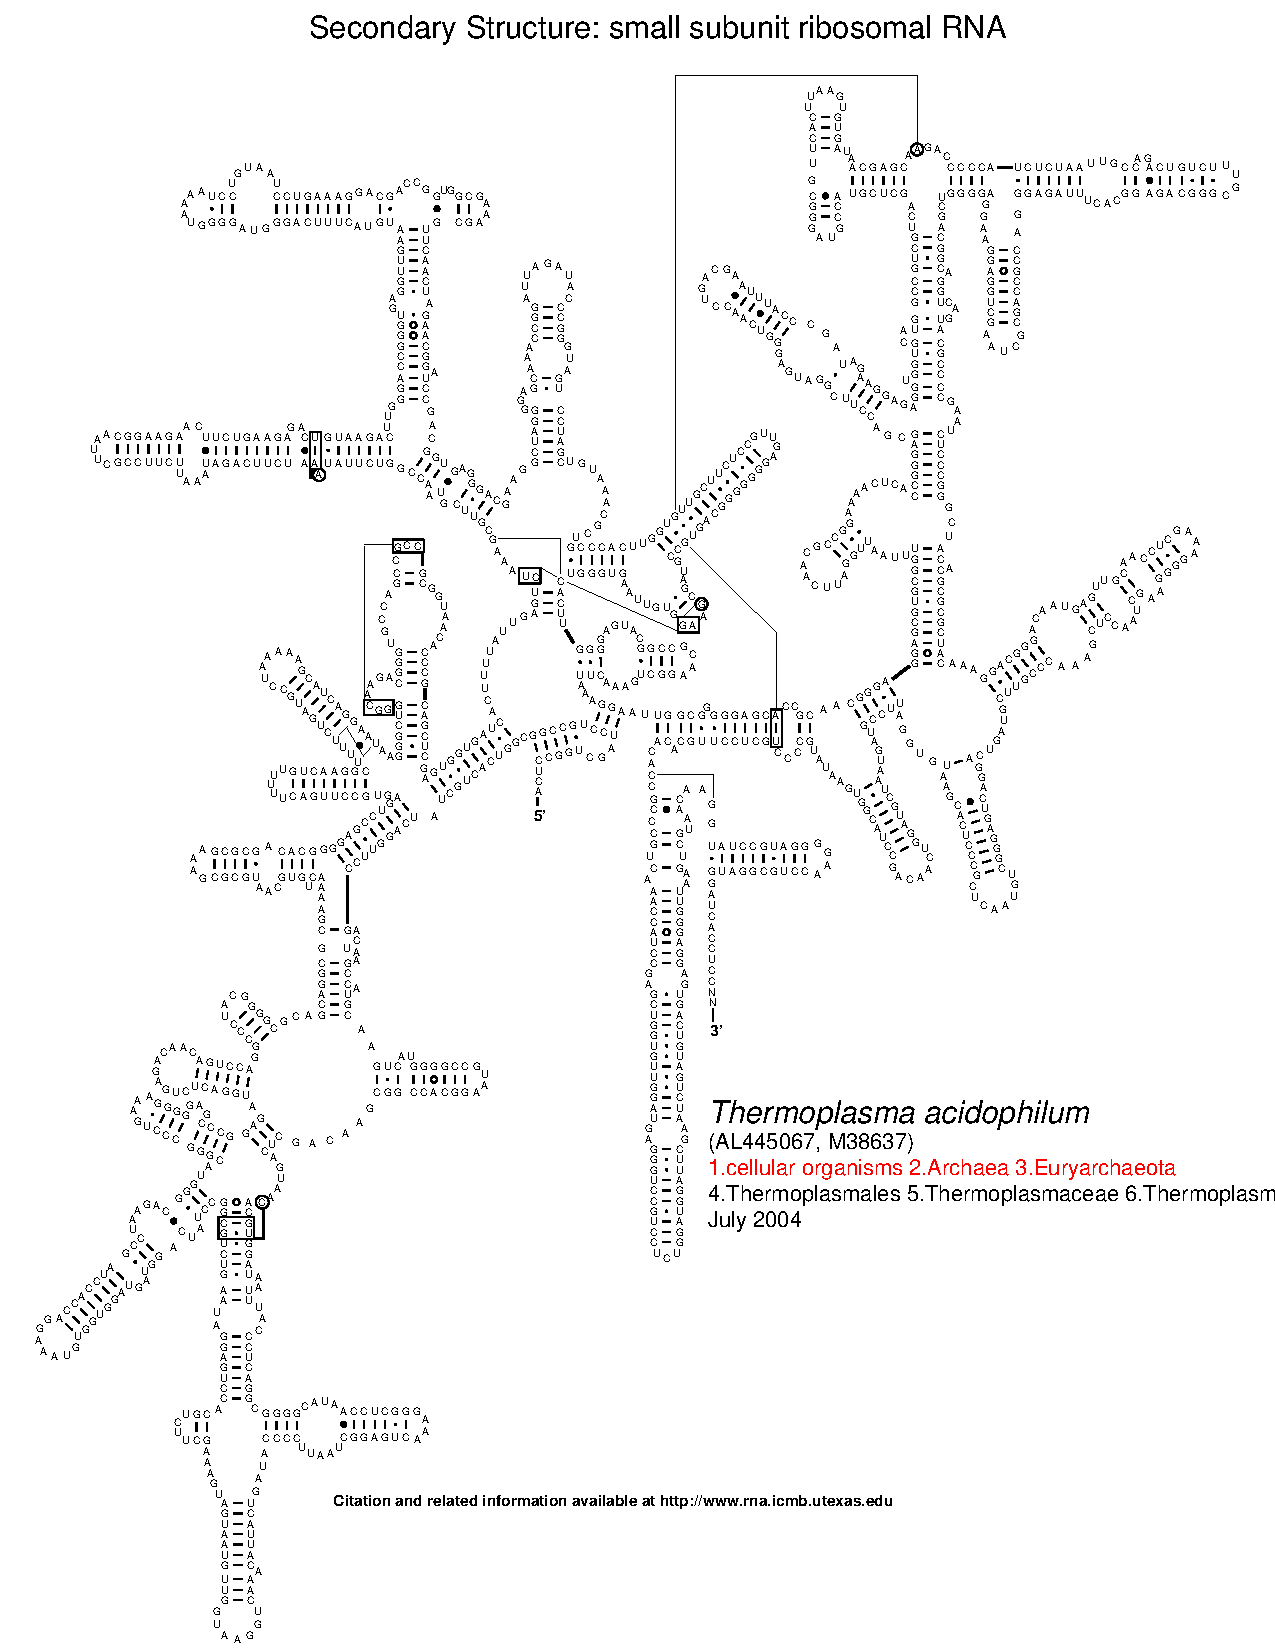
\includegraphics[height=8in]{figs/arc-23}\end{center}\vfill\end{slide}
%%%%%%%%%%%%%%%%%%%%%%%%%%%%%%%%%%%%%%%%%%%%%%%%%%%%%%%%%%%%%%%%%%%%%%%%%%%%%%%%%%%%%%%%%%%%%
\begin{slide}\begin{center}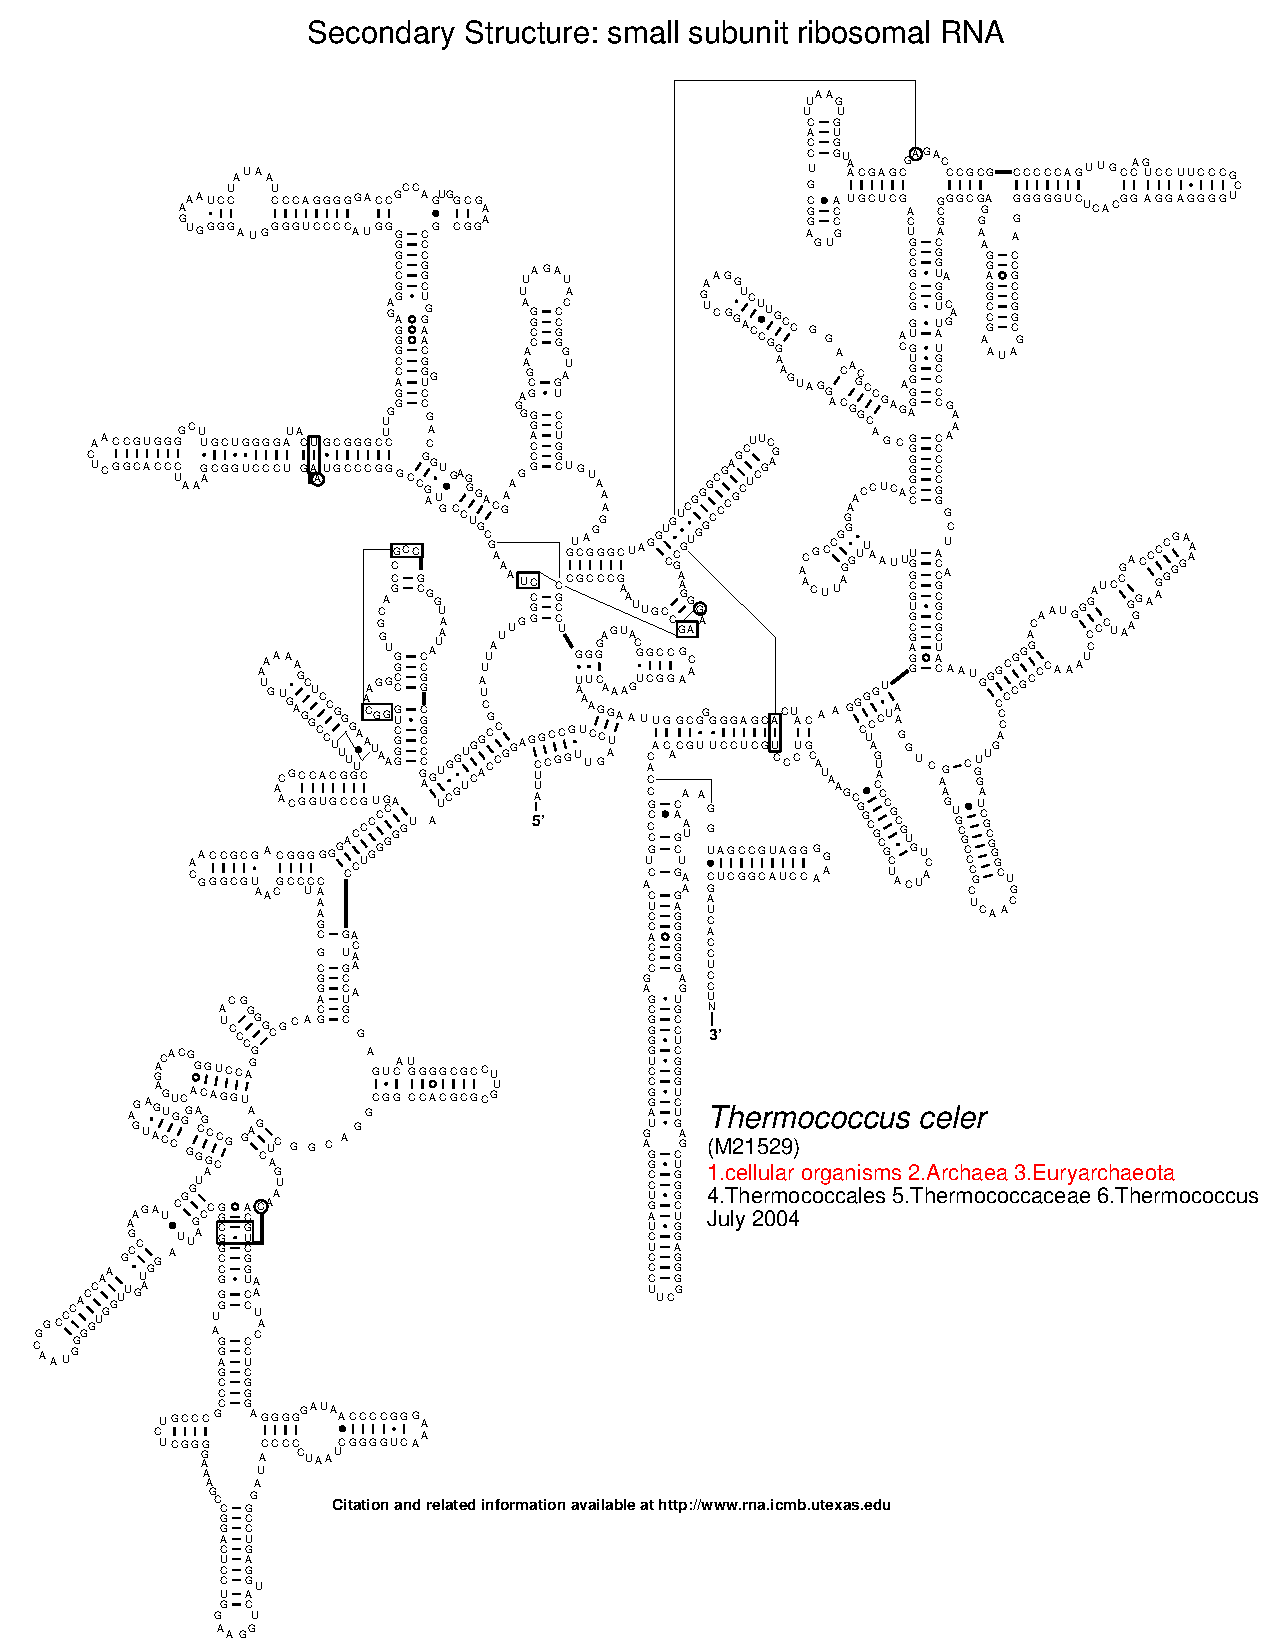
\includegraphics[height=8in]{figs/arc-24}\end{center}\vfill\end{slide}
%%%%%%%%%%%%%%%%%%%%%%%%%%%%%%%%%%%%%%%%%%%%%%%%%%%%%%%%%%%%%%%%%%%%%%%%%%%%%%%%%%%%%%%%%%%%%
\begin{slide}\begin{center}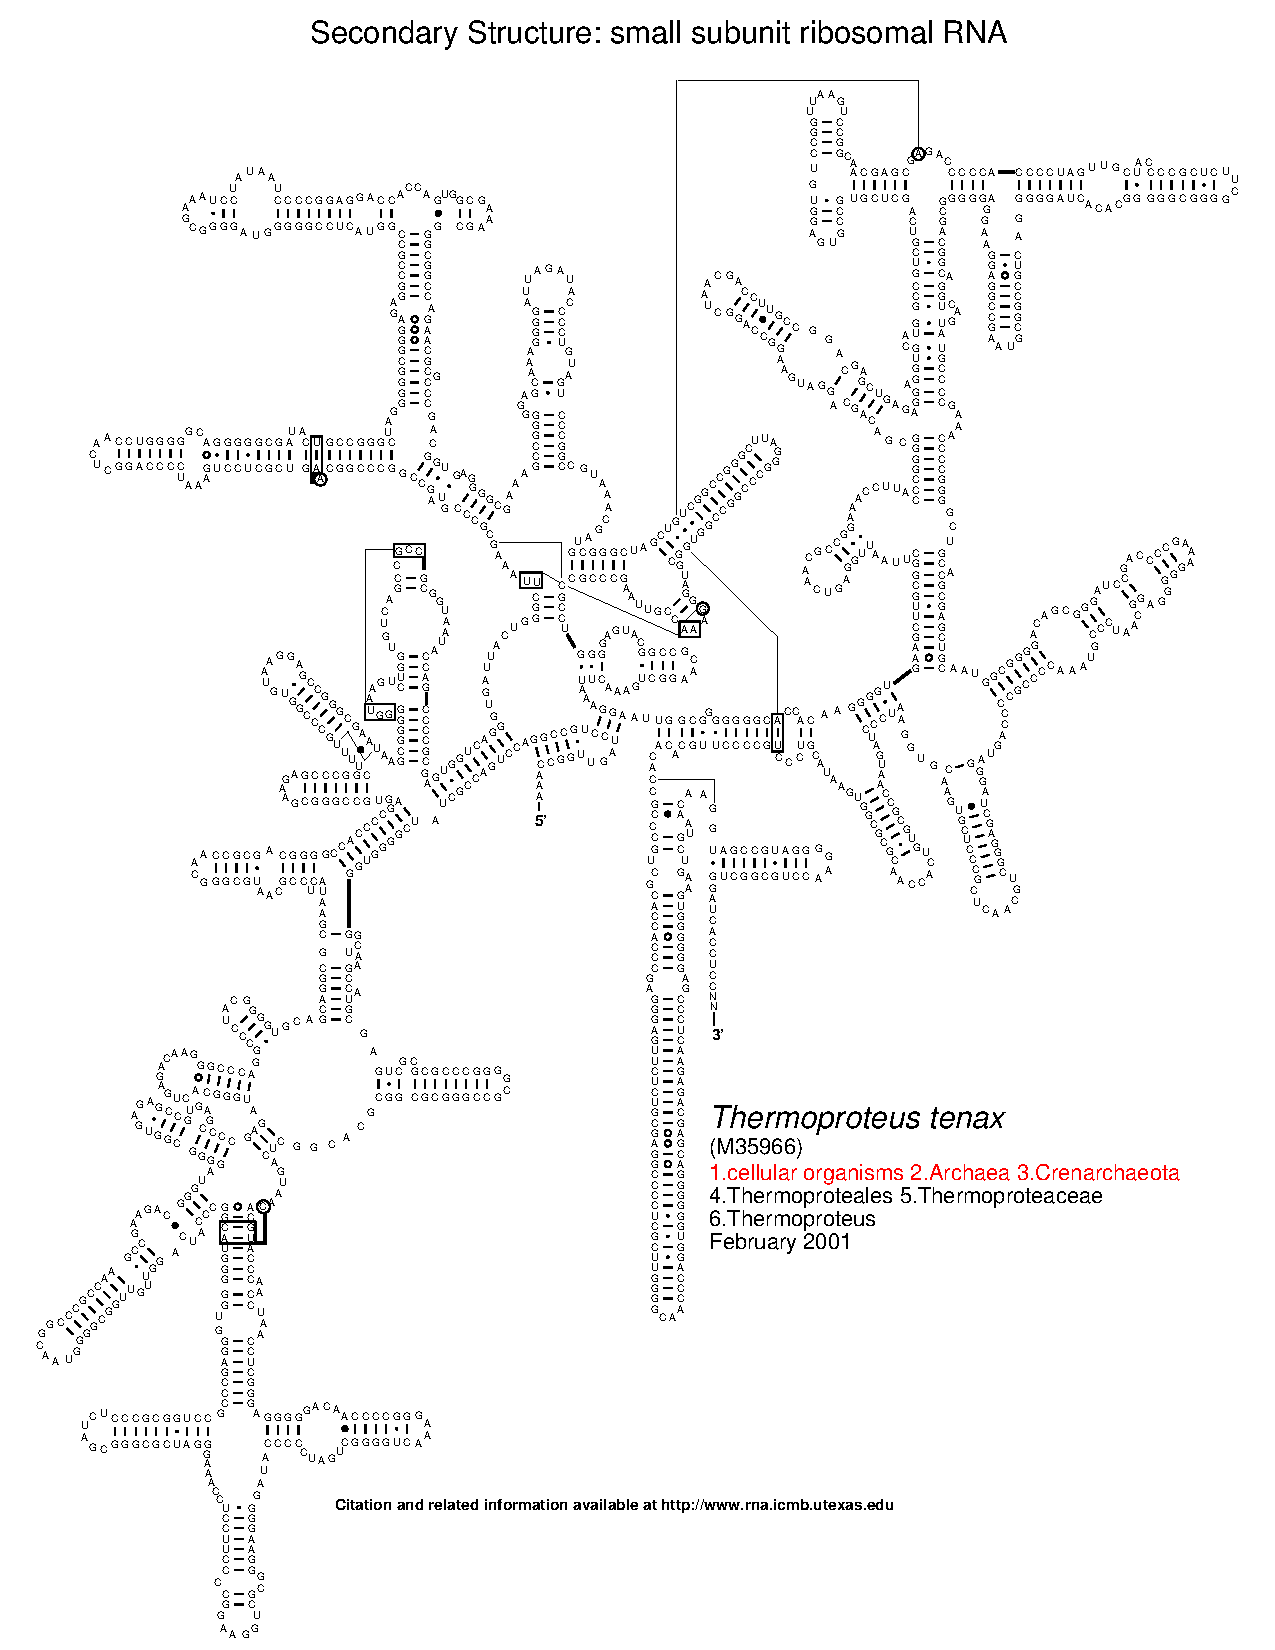
\includegraphics[height=8in]{figs/arc-25}\end{center}\vfill\end{slide}
%%%%%%%%%%%%%%%%%%%%%%%%%%%%%%%%%%%%%%%%%%%%%%%%%%%%%%%%%%%%%%%%%%%%%%%%%%%%%%%%%%%%%%%%%%%%%
\begin{slide}
\begin{center}
\textbf{Phil Hugenholtz's manually created mask}
\end{center}
\small

\begin{center}
\includegraphics[height=7.5in]{figs/lmph-on-1513}

\end{center}
\vfill
\end{slide}
%%%%%%%%%%%%%%%%%%%%%%%%%%%%%%%%%%%%%%%%%%%%%%%%%%%%%%%%%%%%%%%%%%%%%%%%%%%%%%%%%%%%%%%%%%%%%
\begin{slide}
\begin{center}
\textbf{Automatically generated Archaeal mask using CM posterior probabilities}
\end{center}
\small

\begin{center}
\includegraphics[height=7.5in]{figs/inf-lm}

\end{center}
\vfill
\end{slide}
%%%%%%%%%%%%%%%%%%%%%%%%%%%%%%%%%%%%%%%%%%%%%%%%%%%%%%%%%%%%%%%%%%%%%%%%%%%%%%%%%%%%%%%%%%%%%
%%%%%%%%%%%%%%%%%%%%%%%%%%%%%%%%%%%%%%%%%%%%%%%%%%%%%%%%%%%%%%%%%%%%%%%%%%%%%%%%%%%%%%%%%%%%%
\begin{slide}
\begin{center}
\textbf{The manually created mask and automated CM-baseda mask are similar}
\end{center}
\small

\begin{center}
\includegraphics[height=6.5in]{figs/lmph-on-1513}
\includegraphics[height=6.5in]{figs/inf-lm}

\end{center}
\vfill
\end{slide}
%%%%%%%%%%%%%%%%%%%%%%%%%%%%%%%%%%%%%%%%%%%%%%%%%%%%%%%%%%%%%%%%%%%%%%%%%%%%%%%%%%%%%%%%%%%%%
%%%%%%%%%%%%%%%%%%%%%%%%%%%%%%%%%%%%%%%%%%%%%%%%%%%%%%%%%
%%%%%%%%%%%%%%%%%%%%%%%%%%%%%%%%%%%%%%%%%%%%%%%%%%%%%%%%%
%%%%%%%%%%%%%%%%%%%%%%%%%%%%%%%%%%%%%%%%%%%%%%%%%%%%%%%%%%%%%%%%%%%%%%%%%%
\begin{slide}
\begin{center}

\textbf{Automated masking removes the \\ majority of alignment errors}
\end{center}
\medskip
\medskip
\begin{center}

\begin{tabular}{rcr} 
& \multicolumn{1}{c}{alignment} & \multicolumn{1}{c}{time} \\
& \multicolumn{1}{c}{accuracy} & \multicolumn{1}{c}{(sec/seq)} \\ \hline
& \multicolumn{1}{c}{} & \multicolumn{1}{c}{} \\
clustalw & 92.2\% & 30.0 \\ 
& \multicolumn{1}{c}{} & \multicolumn{1}{c}{} \\
HMMs & 96.6\% & 0.08 \\ 
& \multicolumn{1}{c}{} & \multicolumn{1}{c}{} \\
non-banded CMs & 98.1\% & 1321.5 \\ 
& \multicolumn{1}{c}{} & \multicolumn{1}{c}{} \\
HMM banded CMs & 98.1\% & 0.7 \\ %1.1
& \multicolumn{1}{c}{} & \multicolumn{1}{c}{} \\
\textcolor{red}{probabilistically masked} & & \\
\textcolor{red}{HMM banded CMs}           & \textcolor{red}{99.7\%} & \textcolor{red}{1.3} \\ %1.1
& \multicolumn{1}{c}{} & \multicolumn{1}{c}{} \\
\end{tabular}
\end{center}

\center{
{\bf CMs produce alignments that are \\ very similar to manually
  refined alignments.}}

\vfill
\end{slide}
%%%%%%%%%%%%%%%%%%%%%%%%%%%%%%%%%%%%%%%%%%%%%%%%%%%%%%%%%%%%%%%%%%%%%%%%%%
\begin{slide}
\begin{center}
\textbf{SSU-ALIGN: megasequence structural alignment of 16S/18S
    ribosomal RNAs using CMs}
\end{center}

\begin{itemize}
\item Includes Archaeal, Bacterial, and Eukaryotic SSU CMs
\item Structurally aligns sequences at about 1 sequence/second.
\item Can handle up to millions of sequences. 
\item Tutorial on SSU-ALIGN tomorrow.
\end{itemize}

\vfill
\end{slide}
%%%%%%%%%%%%%%%%%%%%%%%%%%%%%%%%%%%%%%%%%%%%%%%%%%%%%%%%%%%%%%%%%%%%
\begin{slide}

\large
\begin{center}
\large{\textbf{Acknowledgements}} \\

\vspace{0.5in}

\normalsize
%\begin{tabular}{llllll}
%Sean Eddy           & & & & & Michael Brent \\ 
%Elena Rivas         & & & & & Jeremy Buhler \\
%Tom Jones           & & & & & Justin Fay \\
%Diana Kolbe         & & & & & Jeff Gordon \\
%Seolkyoung Jung     & & & & & Rob Mitra \\
%Sergi Castellano    & & & & & Gary Stormo \\
%Fred Davis          & & & & & \\
%Lee Henry           & & & & & \\
%Michael Farrar      & & & & & \\
%Travis Wheeler      & & & & & \\
\begin{tabular}{l}
Sean Eddy           \\
Elena Rivas         \\
Travis Wheeler      \\
Tom Jones           \\
Diana Kolbe         \\
Seolkyoung Jung     \\
Fred Davis          \\
Lee Henry           \\
Michael Farrar      \\
\end{tabular}

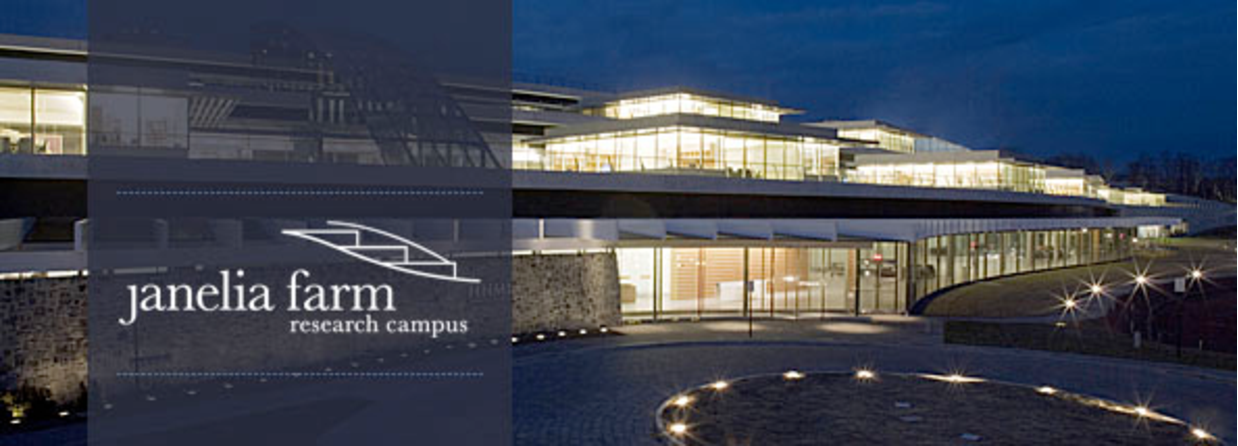
\includegraphics[height=3in]{figs/jfrc-banner1}

\end{center}

\vfill
\end{slide}
%%%%%%%%%%%%%%%%%%%%%%%%%%%%%%%%%%%%%%%%%%%%%%%%%%%%%%%%%%%%%%%
\end{document}

